

\documentclass[handout,compress]{beamer}

\usetheme[block=fill]{metropolis}

\usepackage{graphicx} % Allows including images
\usepackage{amsmath,amsfonts,amsthm,amssymb}
\usepackage{color}
\usepackage{xcolor,cancel}
%\setitemize{label=\usebeamerfont*{itemize item}%
%	\usebeamercolor[fg]{itemize item}
%	\usebeamertemplate{itemize item}}
\definecolor{mDarkBrown}{HTML}{604c38}
\definecolor{mDarkTeal}{HTML}{23373b}
\definecolor{mLightBrown}{HTML}{EB811B}
\definecolor{mMediumBrown}{HTML}{C87A2F}
\definecolor{mygreen}{HTML}{98C2B9}
\definecolor{myyellow}{HTML}{DFD79C}
\definecolor{myblue}{HTML}{8CA7CC}
\definecolor{kern}{HTML}{8CC2B7}

\usepackage{float}
\usepackage{framed}
\usepackage{epsfig}
\usepackage{graphicx}
\usepackage{subcaption}
\usepackage{ulem}
\usepackage{hhline}
\usepackage{multirow}
\usepackage{comment}   
\usepackage{bbm}
\usepackage{tikz}   
\usepackage{ulem}
\def\Put(#1,#2)#3{\leavevmode\makebox(0,0){\put(#1,#2){#3}}}
\newcommand*\mystrut[1]{\vrule width0pt height0pt depth#1\relax}
\newcommand{\eqdef}{\mathbin{\stackrel{\rm def}{=}}}


\newcommand{\bs}[1]{\boldsymbol{#1}}
\newcommand{\bv}[1]{\mathbf{#1}}
\newcommand{\R}{\mathbb{R}}
\newcommand{\E}{\mathbb{E}}

\DeclareMathOperator*{\argmin}{arg\,min}
\DeclareMathOperator*{\argmax}{arg\,max}
\DeclareMathOperator{\nnz}{nnz}
\DeclareMathOperator{\Var}{Var}
\DeclareMathOperator{\sinc}{sinc}
\DeclareMathOperator{\mv}{mv}
\DeclareMathOperator{\sgn}{sgn}
\DeclareMathOperator{\step}{step}
\DeclareMathOperator{\gap}{gap}
\DeclareMathOperator{\poly}{poly}
\DeclareMathOperator{\tr}{tr}
\DeclareMathOperator{\orth}{orth}
\newcommand{\norm}[1]{\|#1\|}
\captionsetup[subfigure]{labelformat=empty}
\captionsetup[figure]{labelformat=empty}
\DeclareMathOperator*{\lmin}{\lambda_{min}}
\DeclareMathOperator*{\lmax}{\lambda_{max}}

\newcommand{\specialcell}[2][c]{%
  \begin{tabular}[#1]{@{}c@{}}#2\end{tabular}}
\newcommand{\specialcellleft}[2][c]{%
\begin{tabular}[#1]{@{}l@{}}#2\end{tabular}
}

\usepackage{tabstackengine}
\stackMath

\newtheorem{claim}[theorem]{Claim}


%----------------------------------------------------------------------------------------
%	TITLE PAGE
%----------------------------------------------------------------------------------------

\title{CS-UY 4563: Lecture 16 \\ Neural Networks cont.}
\author{NYU Tandon School of Engineering, Prof. Christopher Musco}
\date{}

\begin{document}

\begin{frame}
	\titlepage 
\end{frame}

\metroset{titleformat=smallcaps}

\begin{frame}
	\frametitle{lab 6}
	\begin{center}
	Lab \texttt{lab\_mnist\_partial.ipynb} due \textbf{next Thursday, 4/9.}
	\end{center}
	\begin{itemize}
		\item Covers kernel logistic regression and SVMs, which should be useful in many projects. 
		\item Requires \texttt{Tensorflow} (easiest way to load MNIST data). 
	\end{itemize}
\vspace{-1em}
	\begin{center}
	
\includegraphics[width=.5\textwidth]{kerastf.png}
\end{center}
\end{frame}

\begin{frame}
	\frametitle{neural networks}	
	\begin{center}
		\textbf{\alert{Key Concept}}
	\end{center}
	\textbf{Approach in prior classes:}
	\begin{itemize}
		\item Choose good features or a good kernel. 
		\item Use optimization to find best model given those features. 
	\end{itemize}
	\textbf{Neural network approach:}
\begin{itemize}
	\item Learn good features and a good model \emph{simultaneously}. 
\end{itemize}
\end{frame}

\begin{frame}
	\frametitle{model parameters}
	\textbf{Input:} $\vec{x} = x_1, \ldots, x_{N_I}$
	
	\textbf{Model:} $f(\vec{x}, \Theta)$:
	\begin{itemize}
		\item $\vec{z}_H\in \R^{N_H} = \bv{W}_H\vec{x} + \vec{b}_h$.
		\item $\vec{u}_H = [\vec{z}_H > 0]$ 
		\item $z_O \in \R = \bv{W}_O\vec{u}_H + b_O$
		\item ${u}_O = [{z}_O > 0]$
	\end{itemize}

	\textbf{Parameters:} $\Theta = [\bv{W}_H\in \R^{N_H\times N_I}, \vec{b}_H\in \R^{N_H} , \bv{W}_O\in \R^{1\times N_H}, {b}_O\in \R]$.
	
	\begin{center}
		$\bv{W}_H$, $\bv{W}_O$ are \emph{weight matrices} and $\vec{b}_H$, ${b}_O$ are \emph{bias} terms that account for the intercepts of our linear functions.  
	\end{center}
\end{frame}

\begin{frame}
	\frametitle{two-layer (sigmoid) perceptron}
	Function $f$ which maps $\vec{x}$ to a class label $u_O$.

	\begin{center}
		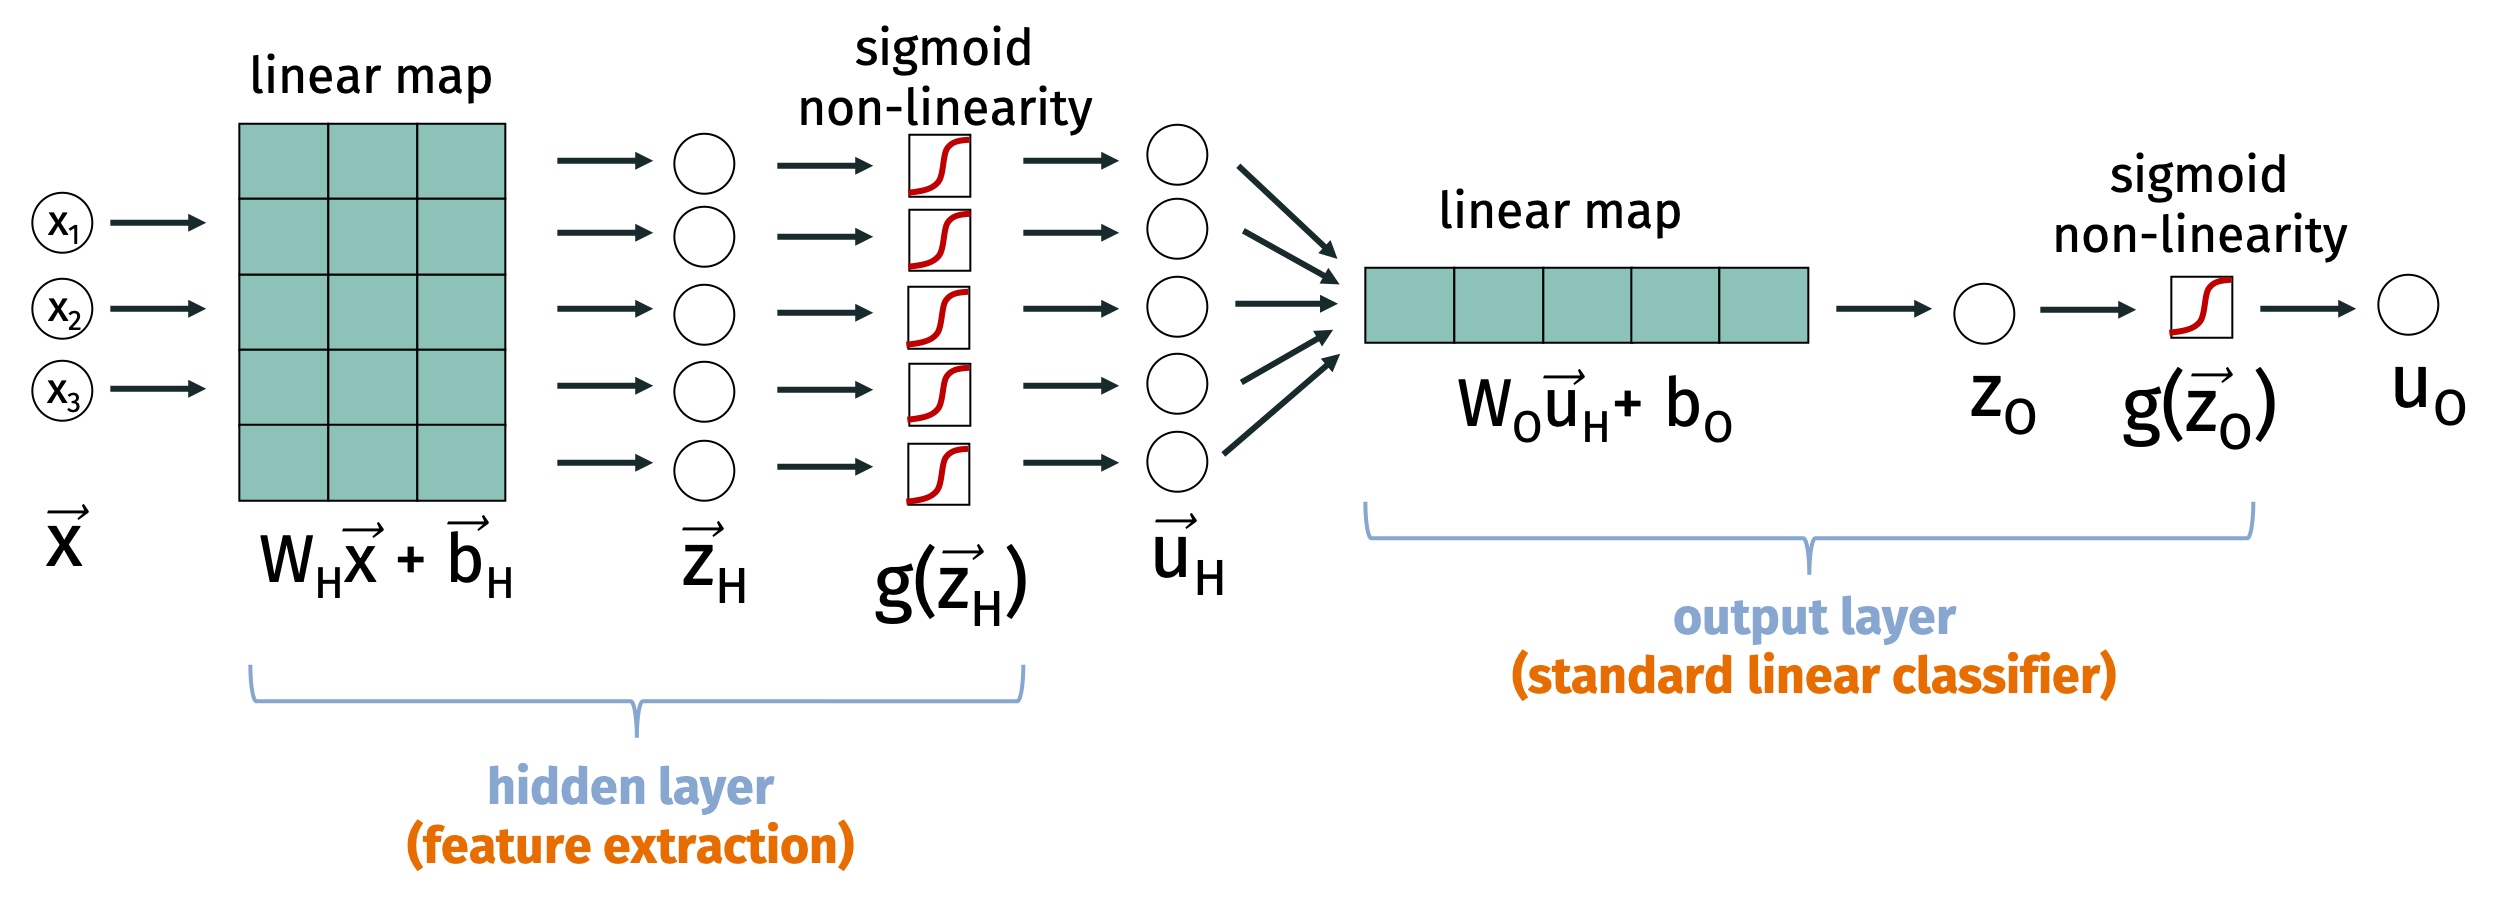
\includegraphics[width=\textwidth]{neural_net_arch.png}
	\end{center}	
\end{frame}

\begin{frame}
	\frametitle{feature extraction}
	Features learned using step-function activation are binary, depending on which side of a set of \emph{learned} hyperplanes each point lies on. 
	\begin{center}
		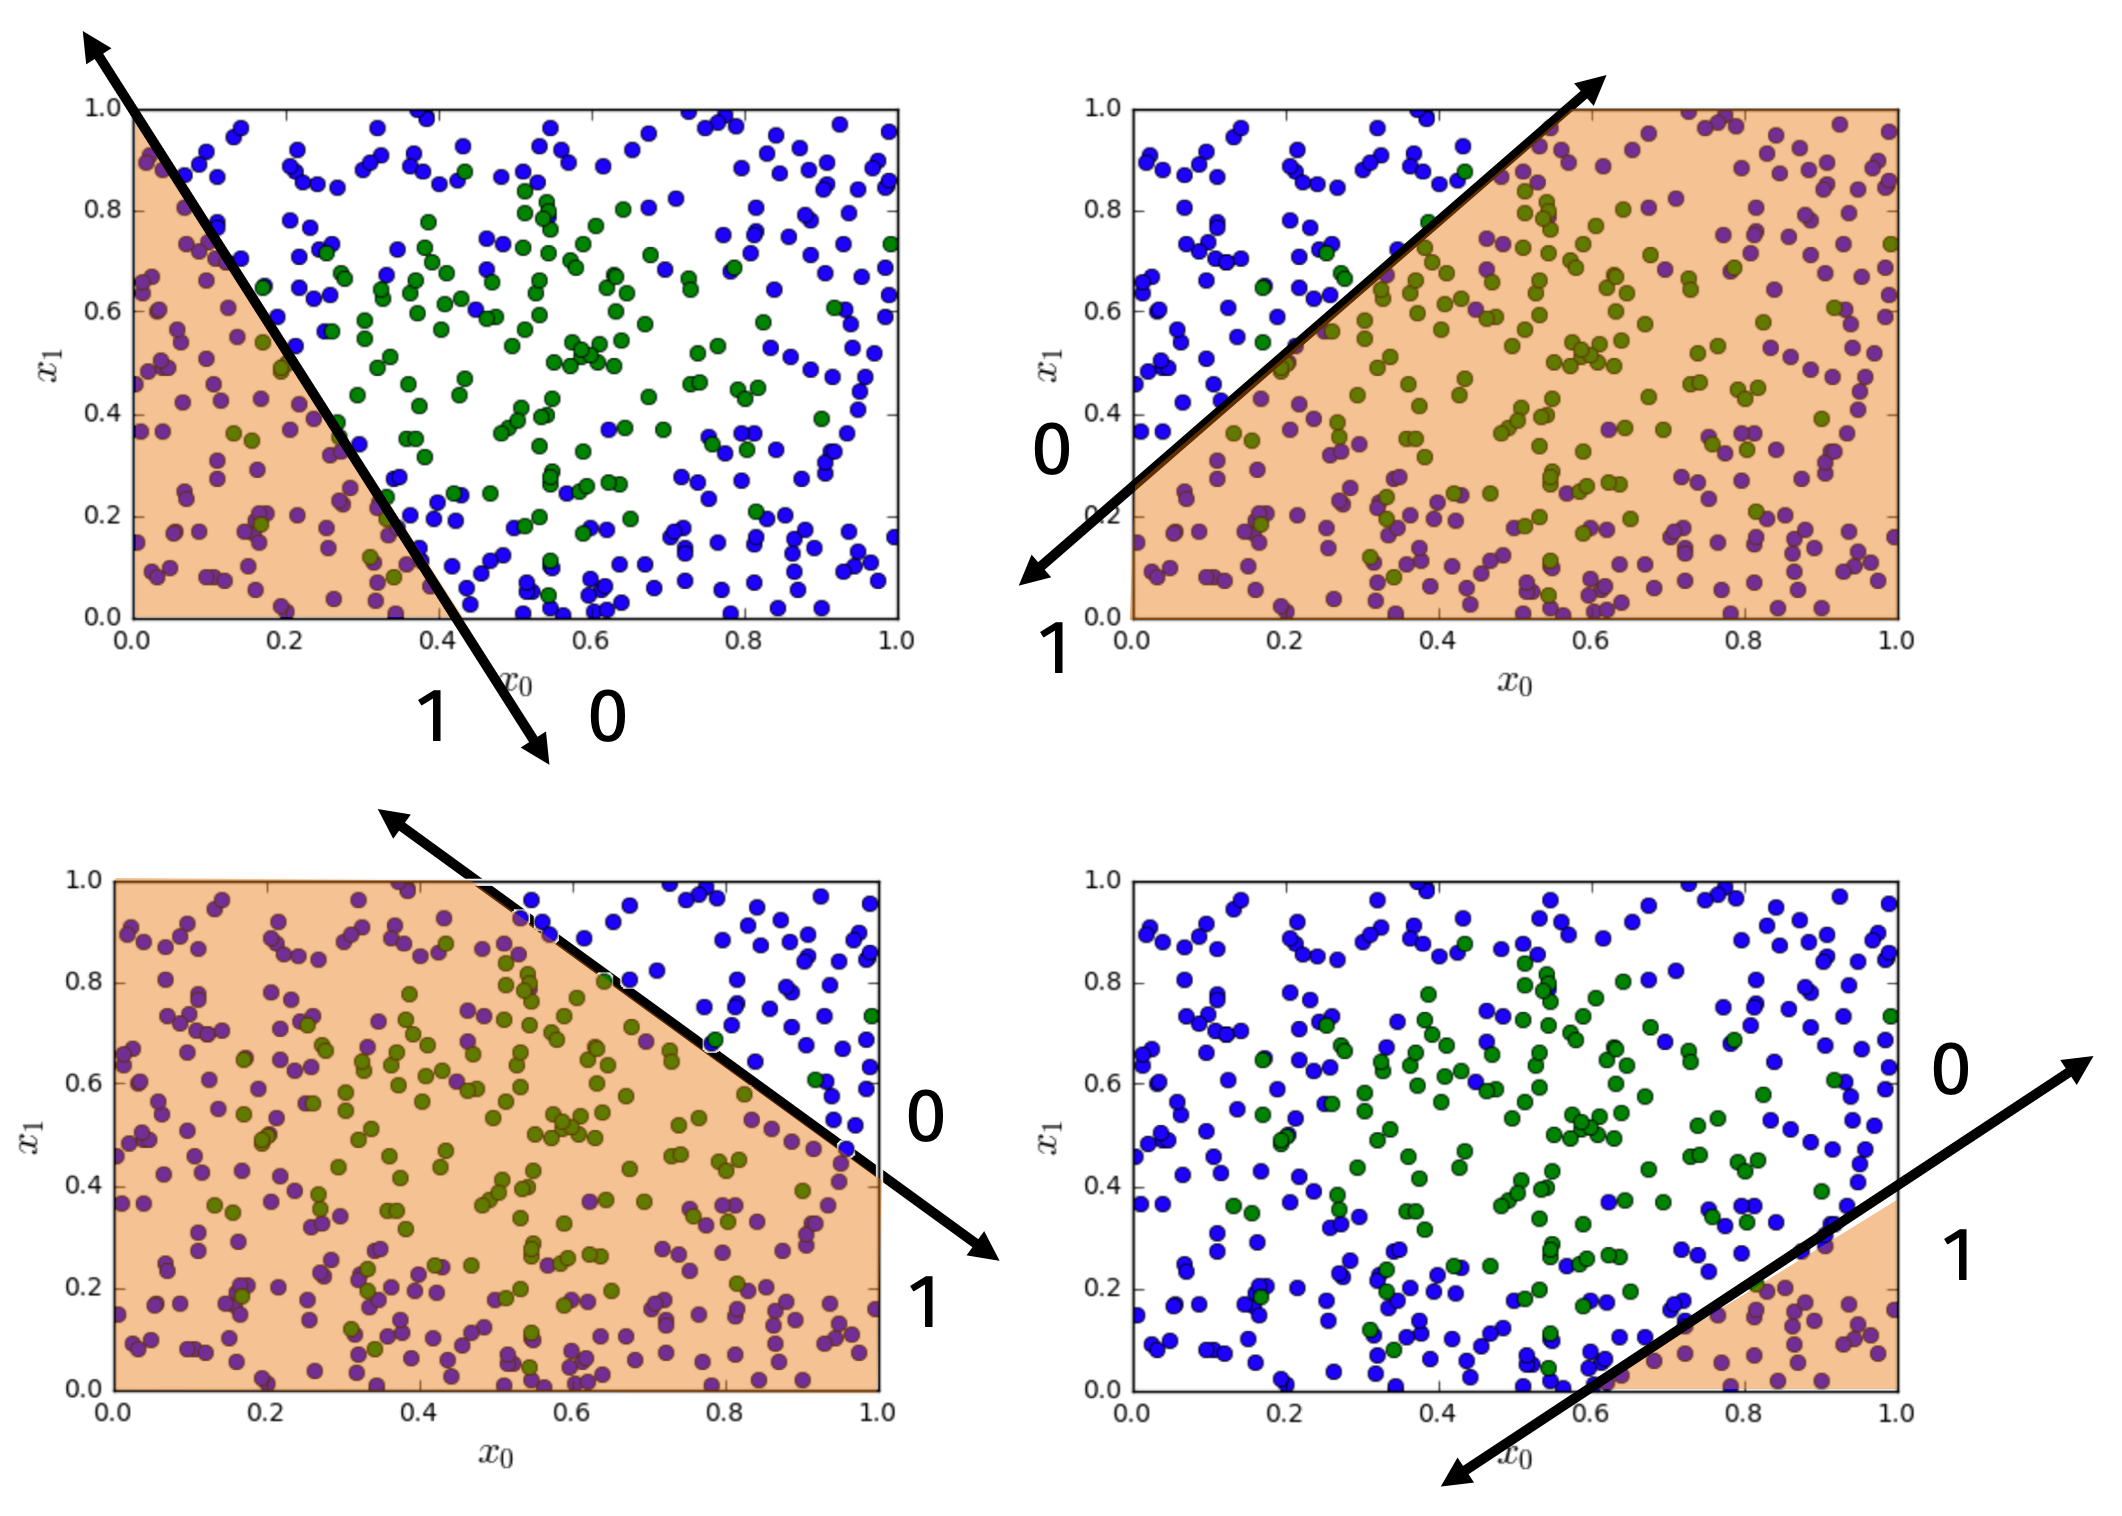
\includegraphics[width=.8\textwidth]{hard_features.png}
	\end{center}	
\end{frame}

\begin{frame}
	\frametitle{feature extraction}
	Features learned using sigmoid activation are real valued in $[0,1]$. Mimic binary features.  
	\begin{center}
		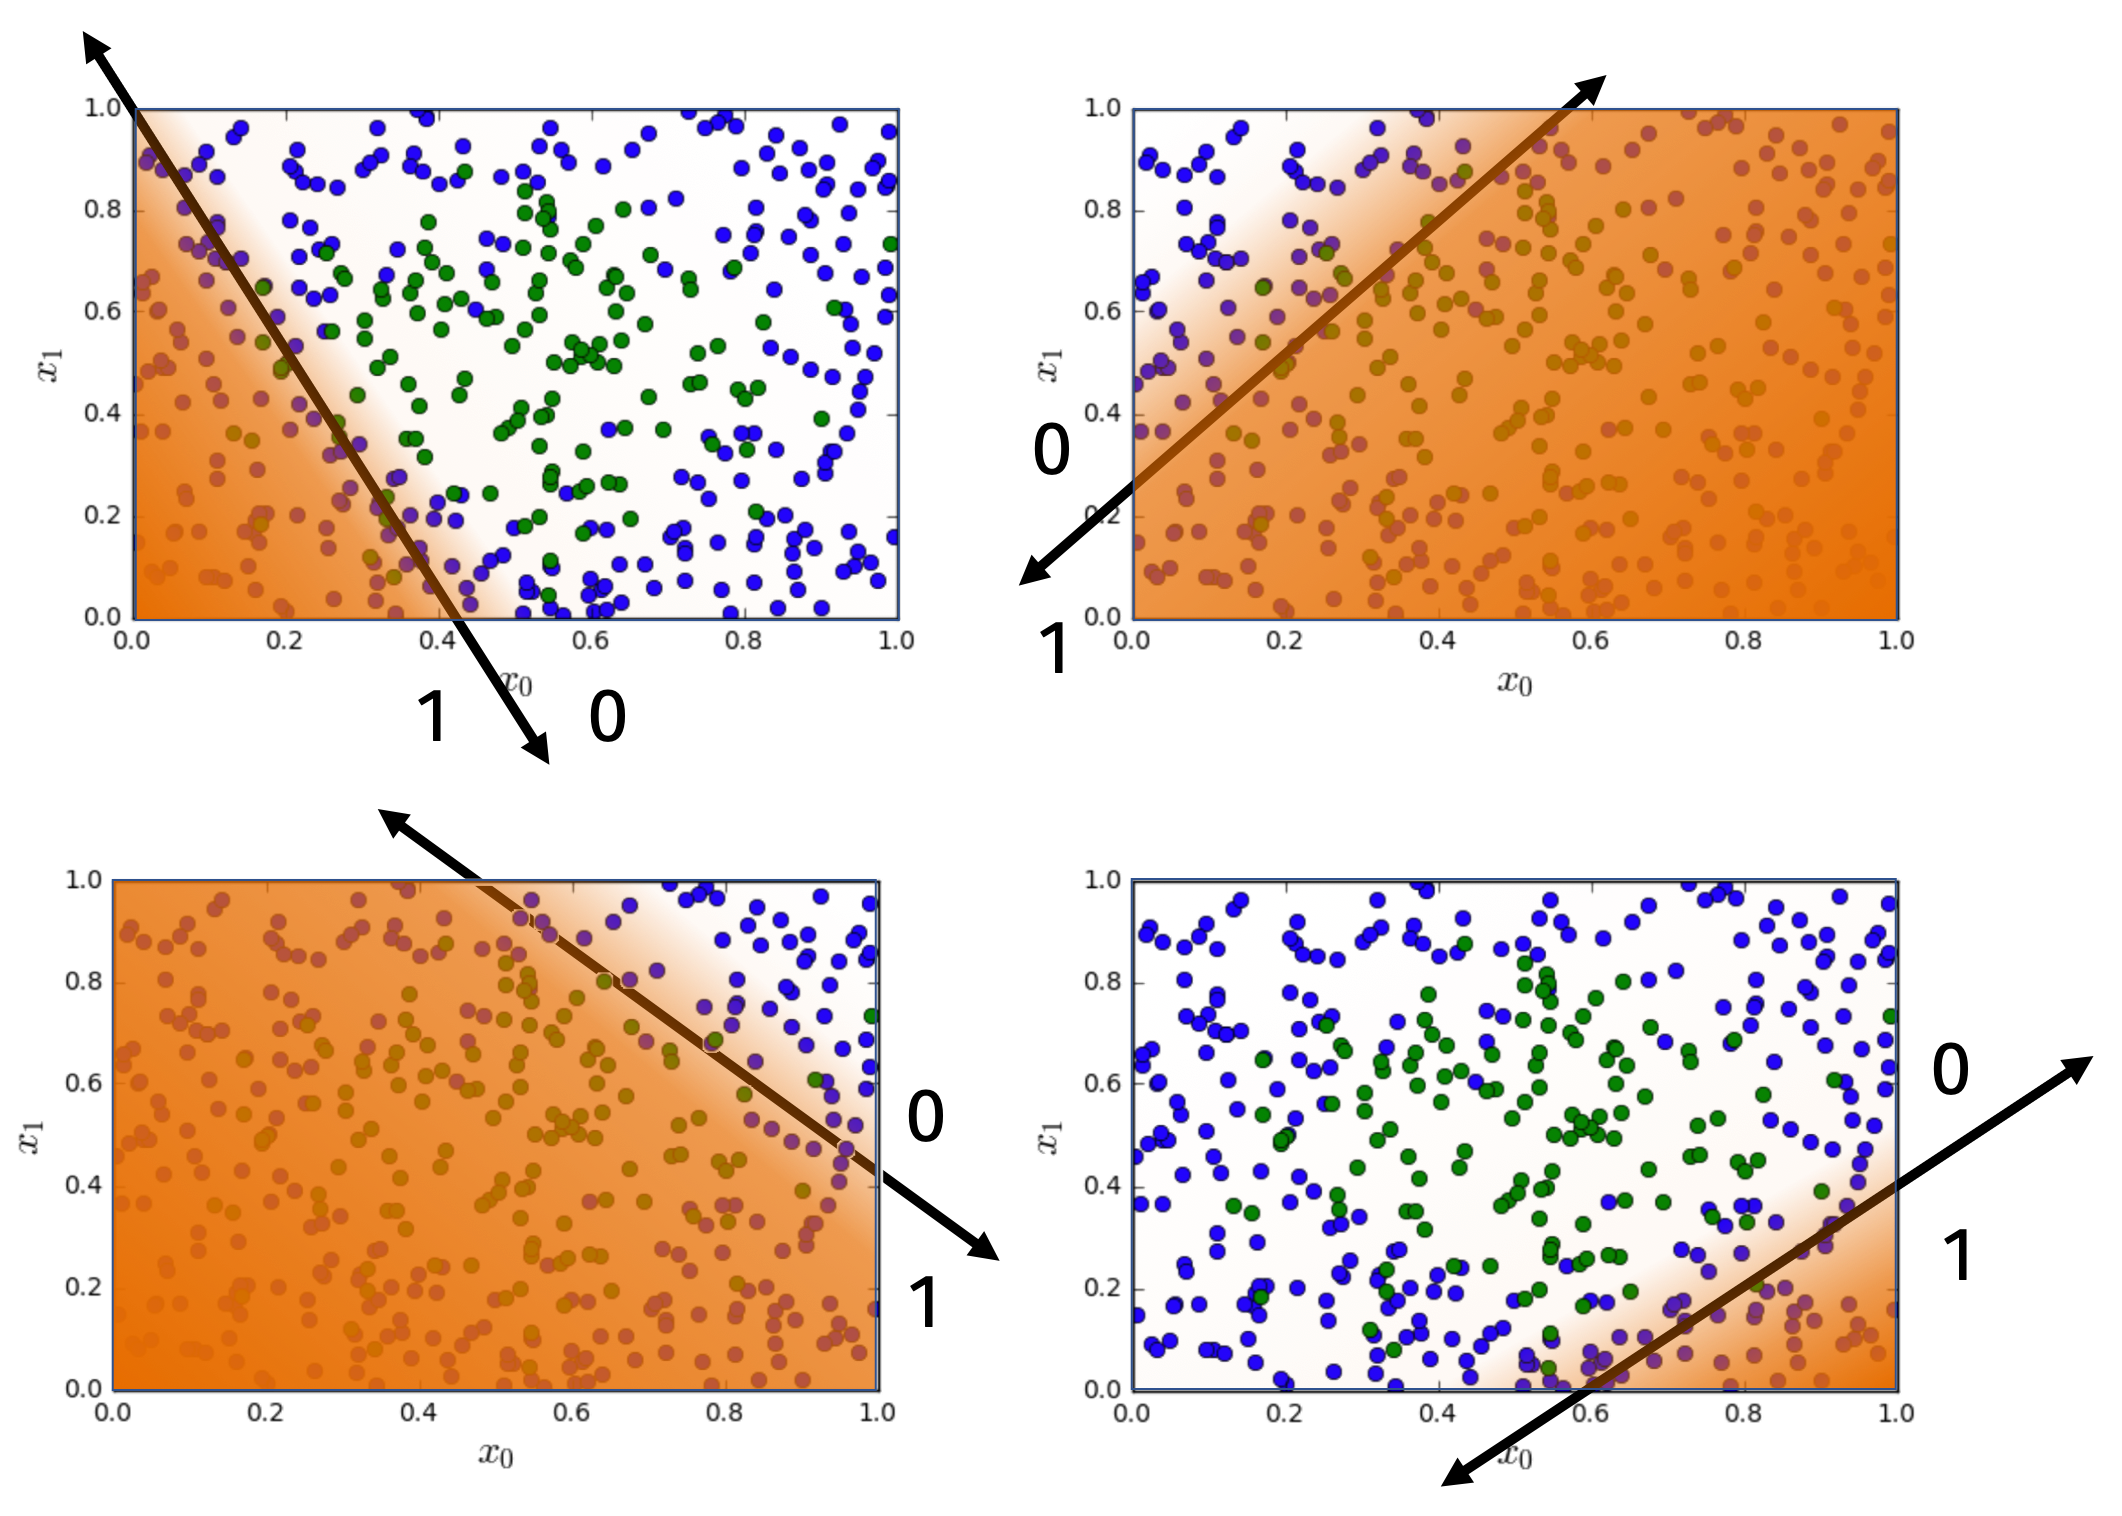
\includegraphics[width=.8\textwidth]{soft_features.png}
	\end{center}	
\end{frame}

\begin{frame}
	\frametitle{hyperparameters}
	\textbf{Things we can change in this basic classification network:}
	\begin{itemize}
		\item More or less hidden variables.
		\item Different non-linearity/activation function.
		\item Different loss function (more on that next class). 
		\item More hidden layers (allows for learning hierarchical features).
	\end{itemize}
	\begin{center}
		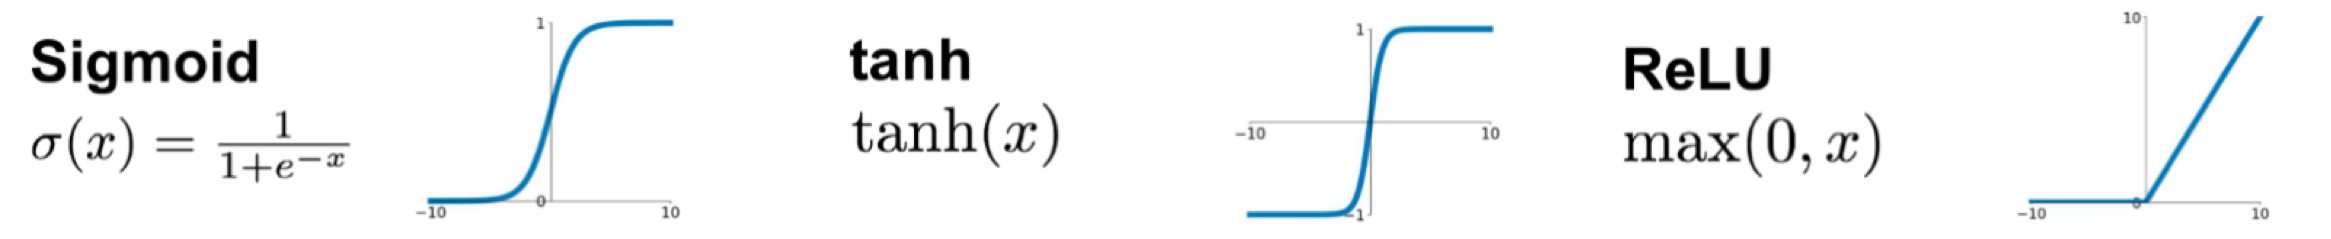
\includegraphics[width=\textwidth]{activation_functions.png}
	\end{center}
\end{frame}


\begin{frame}
	\frametitle{notation}
	\textbf{Another common diagram for a 2-layered network:}
	\begin{center}
		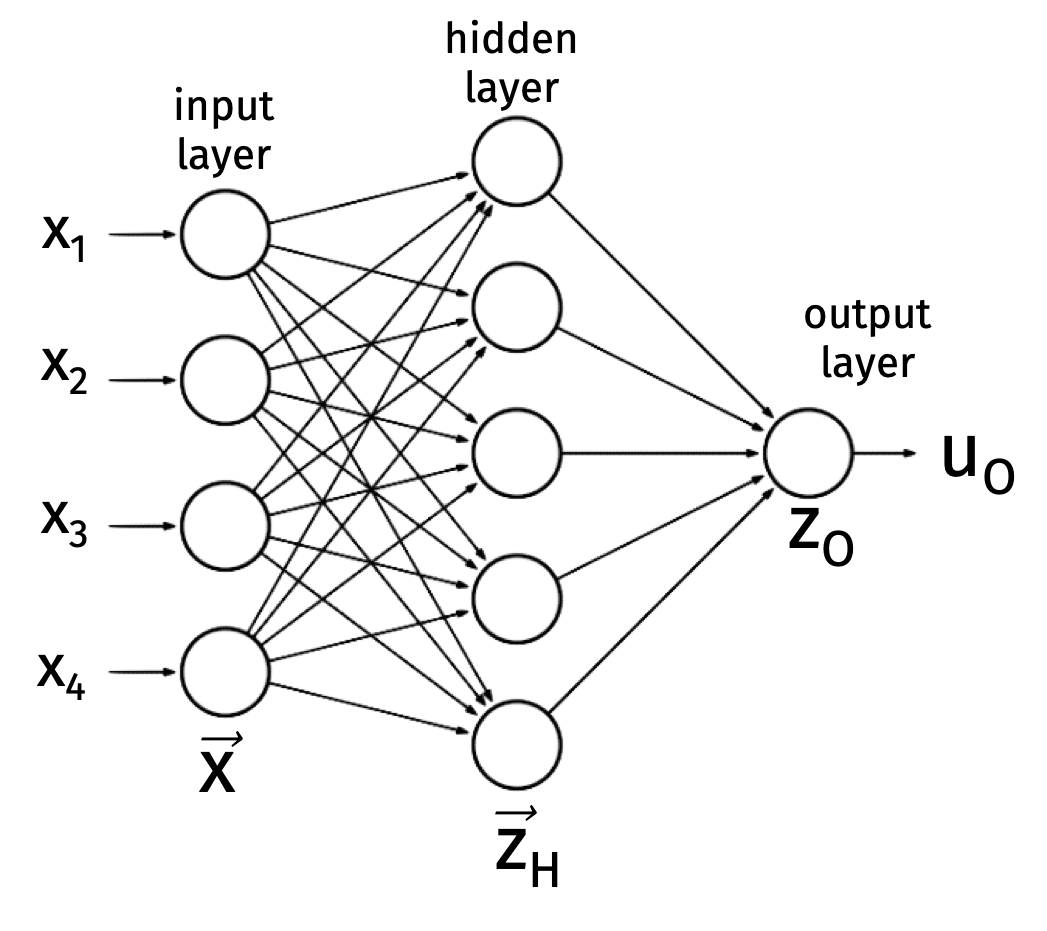
\includegraphics[width=.6\textwidth]{noweights.png}
	\end{center}
\end{frame}

\begin{frame}
	\frametitle{notation}
	\textbf{Neural network math:}
	\begin{center}
		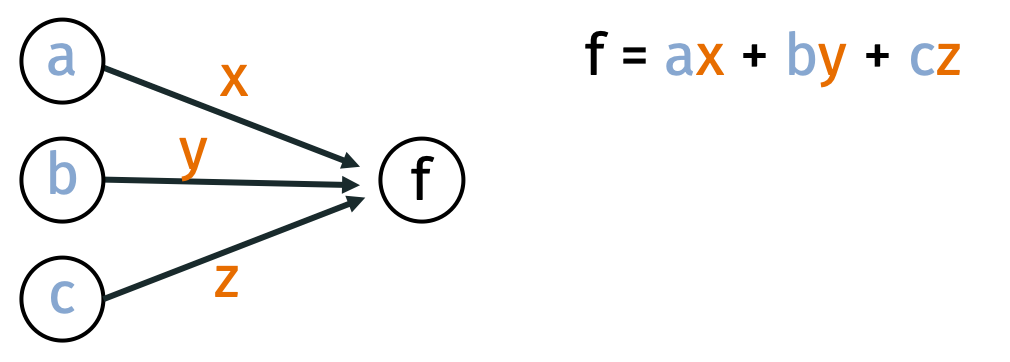
\includegraphics[width=.6\textwidth]{neural_math.png}
	\end{center}
\end{frame}

\begin{frame}
	\frametitle{notation}
	\textbf{How to interpret:}
	\vspace{-1em}
	\begin{center}
		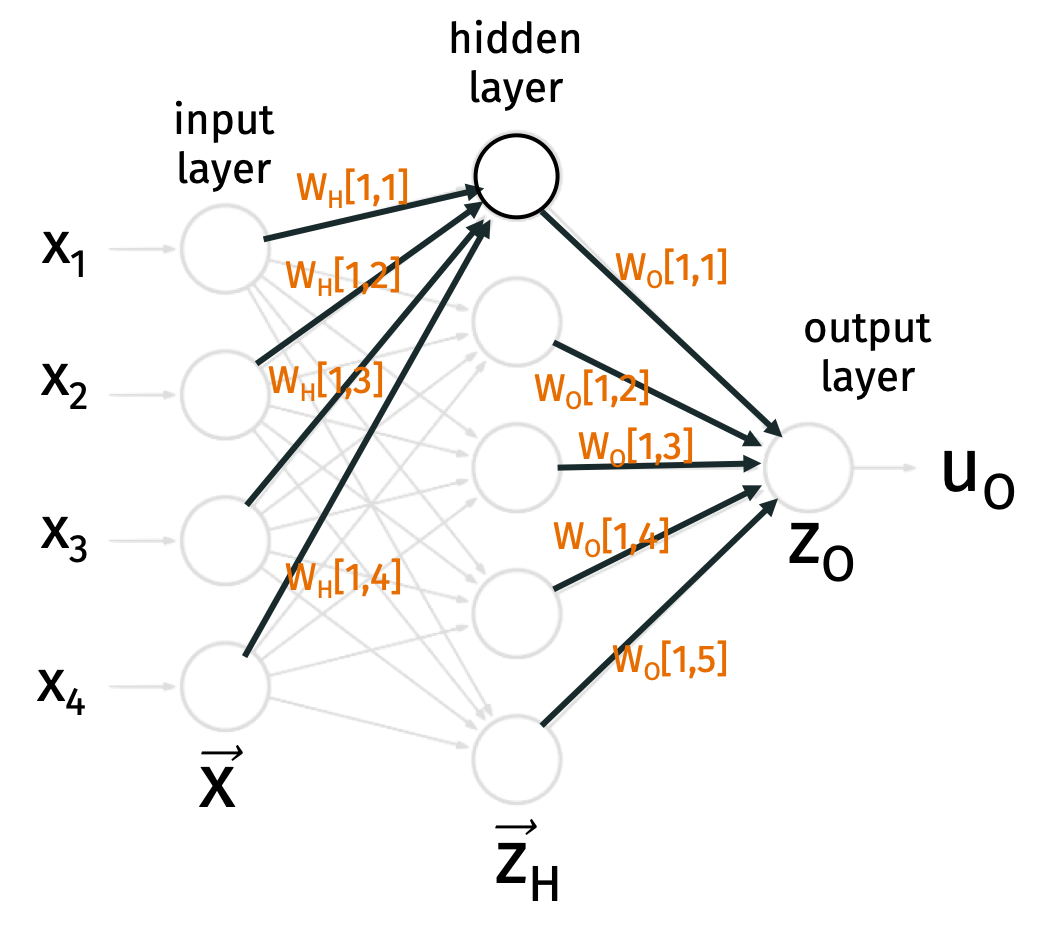
\includegraphics[width=.6\textwidth]{weights1.png}
	\end{center}
\vspace{-1.5em}
$\bv{W}_H$ and $\bv{W}_O$ are our weight matrices from before. 

\textbf{Note:} This diagram does not explicitly show the \emph{bias terms} or the \emph{non-linear activation functions}. 
\end{frame}

\begin{frame}
	\frametitle{notation}
	\textbf{How to interpret:}
	\vspace{-1em}
	\begin{center}
		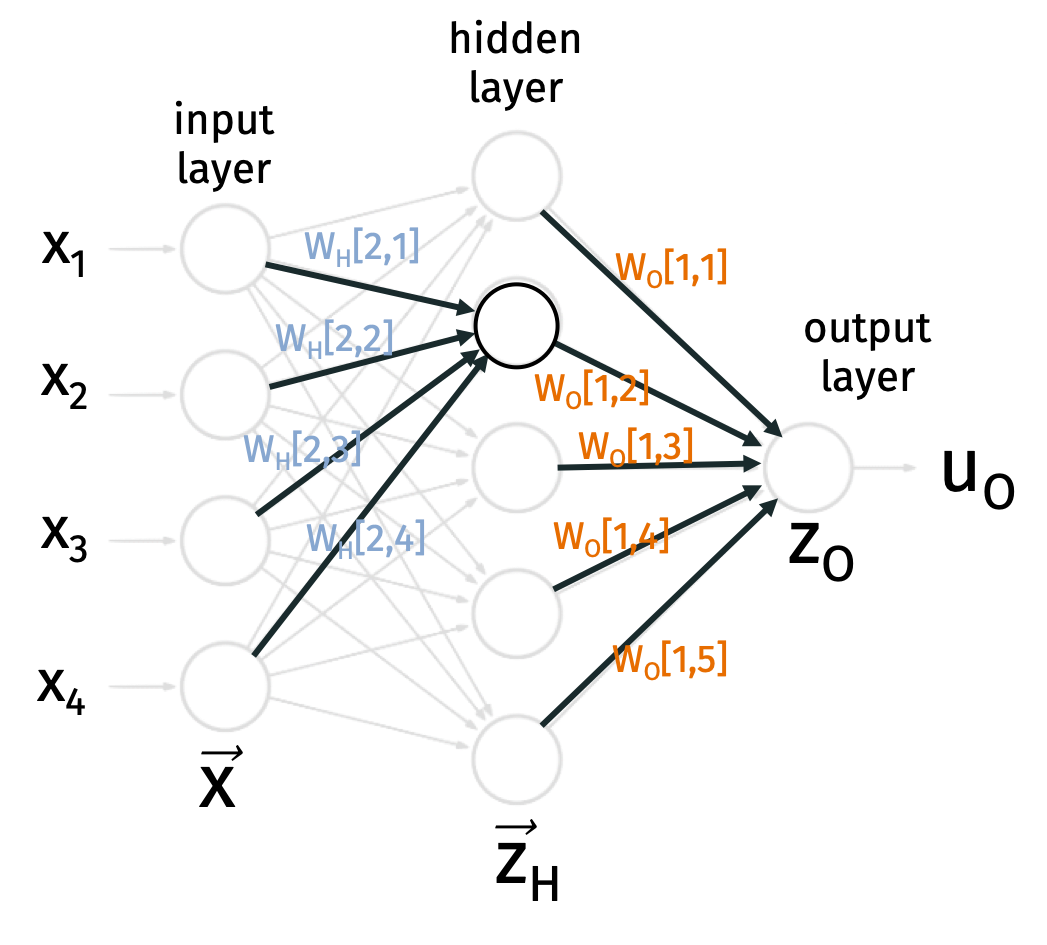
\includegraphics[width=.6\textwidth]{weights2.png}
	\end{center}
\vspace{-1.5em}
$\bv{W}_H$ and $\bv{W}_O$ are our weight matrices from before. 

\small{
\textbf{Note:} This diagram depicts a network with \textbf{``fully-connected''} layers. Every variable in layer $i$ is connected to every variable in layer $i + 1$.}
\end{frame}

\begin{frame}
	\frametitle{architecture visualization}
	\small
 	Effective way of visualize ``architecture'' of a neural network:
	\begin{center} 
		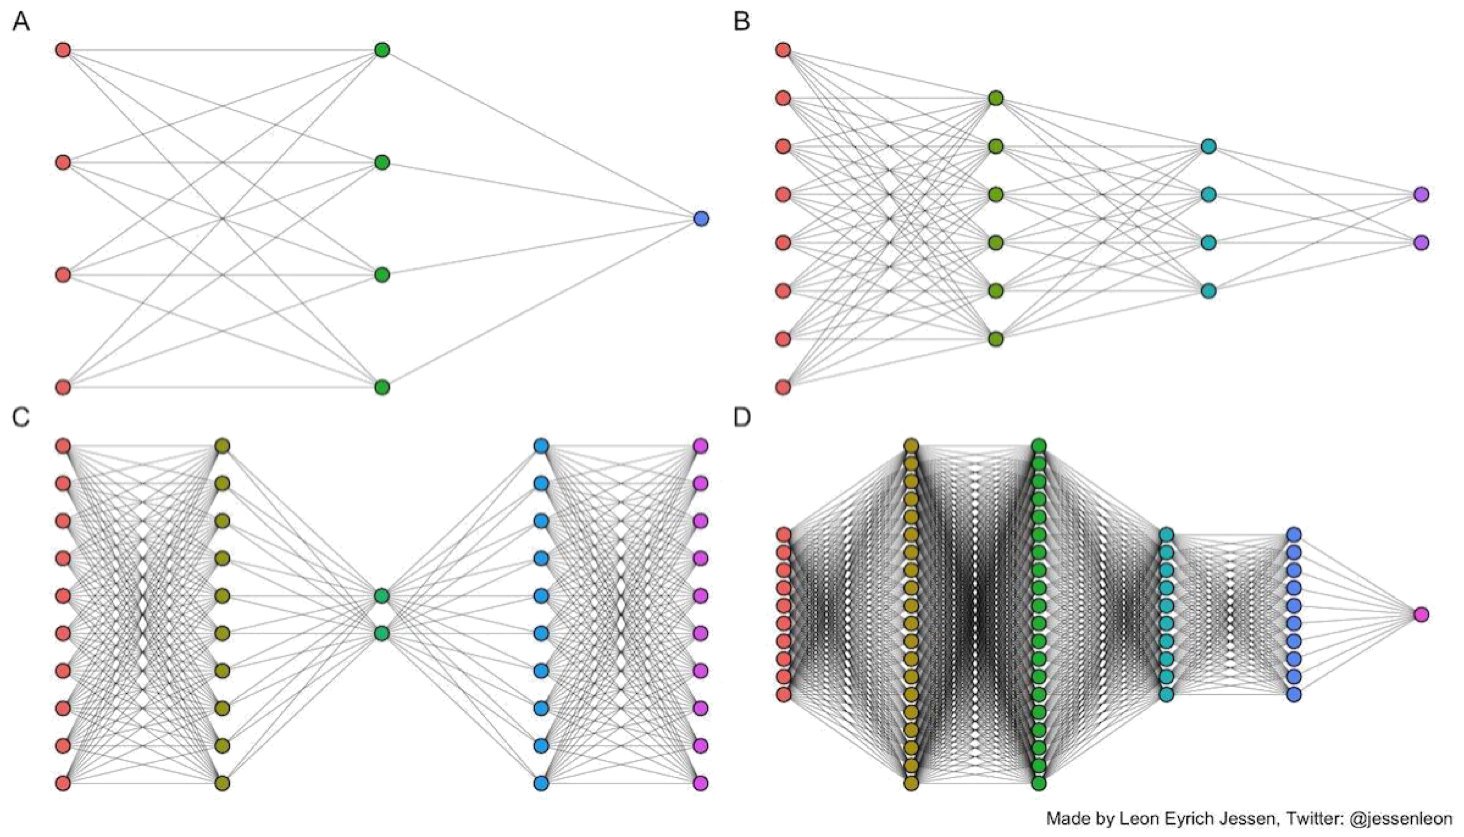
\includegraphics[width=.8\textwidth]{arch_diffs.png}
	\end{center}
Visualize number of variables, types of connections, number of layers and their relative sizes.

These are all \textbf{feedforward} neural networks. No backwards (\textbf{recurrent}) connections.
\end{frame}

\begin{frame}[standout]
	some history and motivation
\end{frame}

\begin{frame}
	\frametitle{connection to biology}
	\small
	\textbf{Simplified model of the brain:}
	\begin{columns}
		\begin{column}{.55\textwidth}
			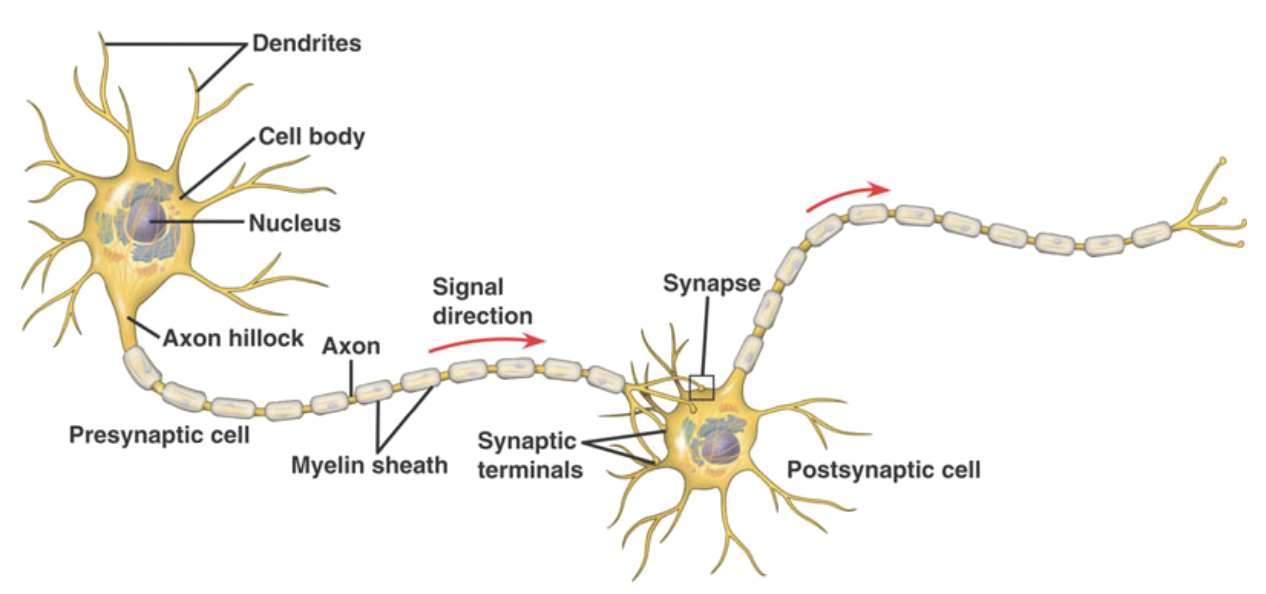
\includegraphics[width=\textwidth]{neurons.png}
		\end{column}
		\begin{column}{.45\textwidth}
			\textbf{Dendrites}: Input electrical current from other neurons.
			
			\textbf{Axon}: Output electrical current to other neurons.
			
			\textbf{Synapse}: Where these two connect.
		\end{column}
	\end{columns}
	A neuron ``fires'' (outputs non-zero electric charge) if it receives enough \emph{cumulative electrical input} from \emph{all neurons connected to it}. 
	\begin{center}
		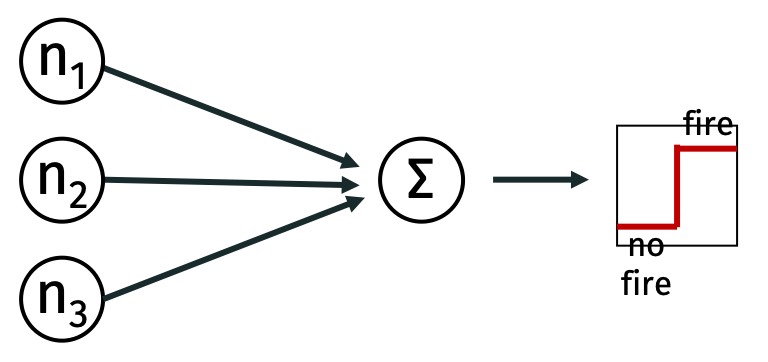
\includegraphics[width=.4\textwidth]{neural_model.png}
	\end{center}
	Output charge can be positive \emph{or} negative (excitatory vs. inhibitory). 
\end{frame}

\begin{frame}
	\frametitle{connection to biology}
	\textbf{Inspired early work on neural networks:}
	\begin{itemize}
		\item 1940s Donald Hebb proposed a Hebbian learning rule for how brains neurons change over time to allow learning.
		\item 1950s Frank Rosenblatt's Perceptron is one of the first ``artifical'' neural networks.
		\item Continued work throughout the 1960s. 
	\end{itemize}
\textbf{Main issue with neural network methods:} They are \emph{hard to train}. Generally require a lot of computation power. Also pretty finicky: user needs to be careful with initialization, regularization, etc. when training.  Often requires a lot of experimentation to get right.
\end{frame}

\begin{frame}
	\frametitle{early neural network explosion}
	Around 1985 several groups (re)-discovered the \textbf{backpropagation algorithm} which allows for efficient training of neural nets via \textbf{gradient descent}. Along with increased computational power this lead to a resurgence of interest in neural network models. 
	\begin{center}		
		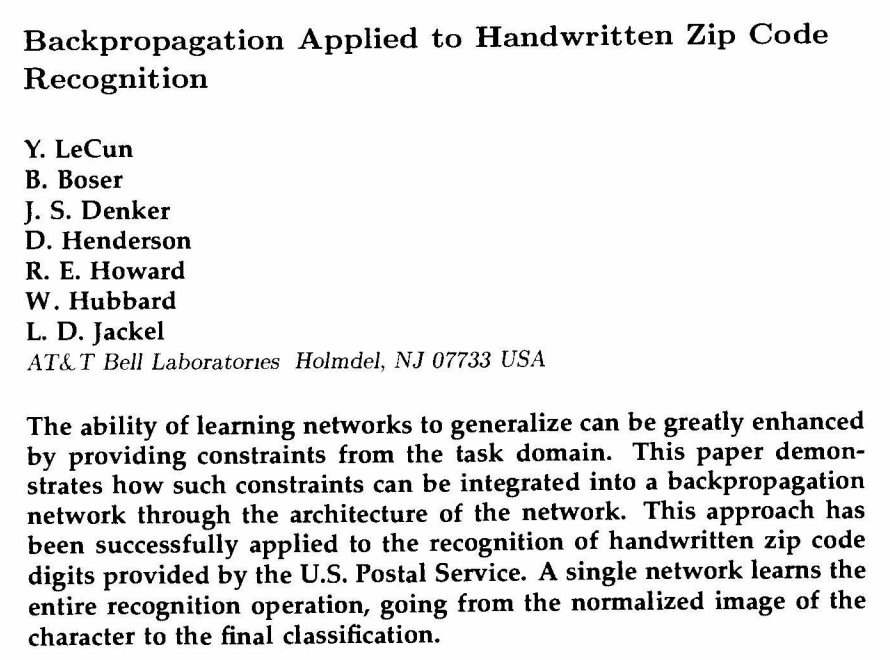
\includegraphics[width=.5\textwidth]{mnistbackprop.png}
	\end{center}
Very good performance on problems like digit recognition.
\end{frame}

\begin{frame}
	\frametitle{neural network decline}
	In the 1990s and early 2000s, kernel methods, SVMs, and probabilistic methods began to dominate the literature in machine learning:
	\begin{itemize}
		\item Work well ``out of the box".
		\item Relatively easy to understand theoretically.
		\item Not too computationally expensive for moderately sized datasets. 
	\end{itemize}
\textbf{Fun blog post to check out from 2005:} \url{http://yaroslavvb.blogspot.com/2005/12/trends-in-machine-learning-according.html}
\end{frame}

\begin{frame}
	\frametitle{neural network decline}
		\footnotesize
	Finding trends in machine learning by search papers in Google Scholar that match a certain keyword:
	\begin{center}		
		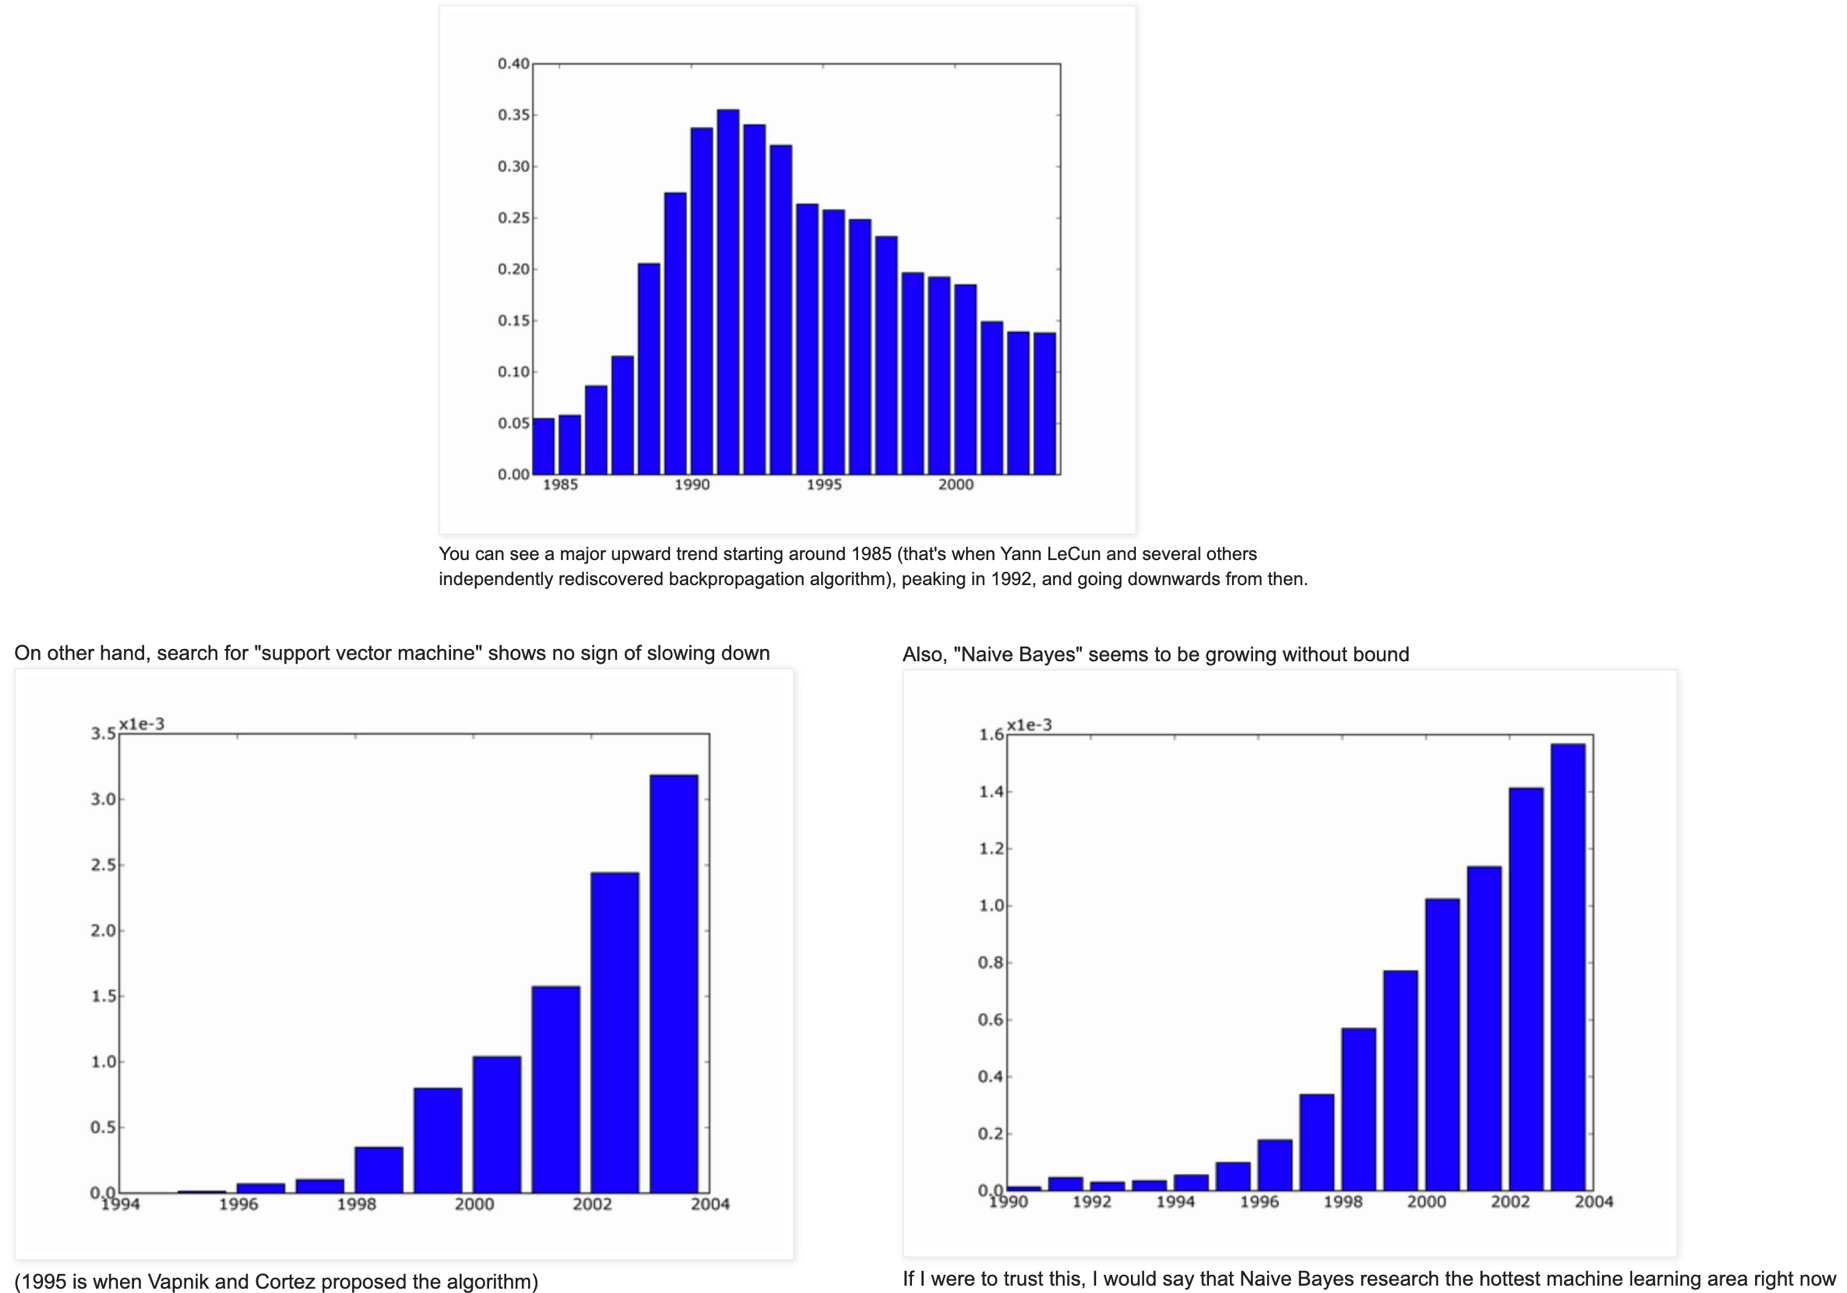
\includegraphics[width=.9\textwidth]{trends.png}
	\end{center}
\end{frame}

\begin{frame}
	\frametitle{modern neural network resurgence}
	In recent years this trend completely turned around:
	\begin{center}
		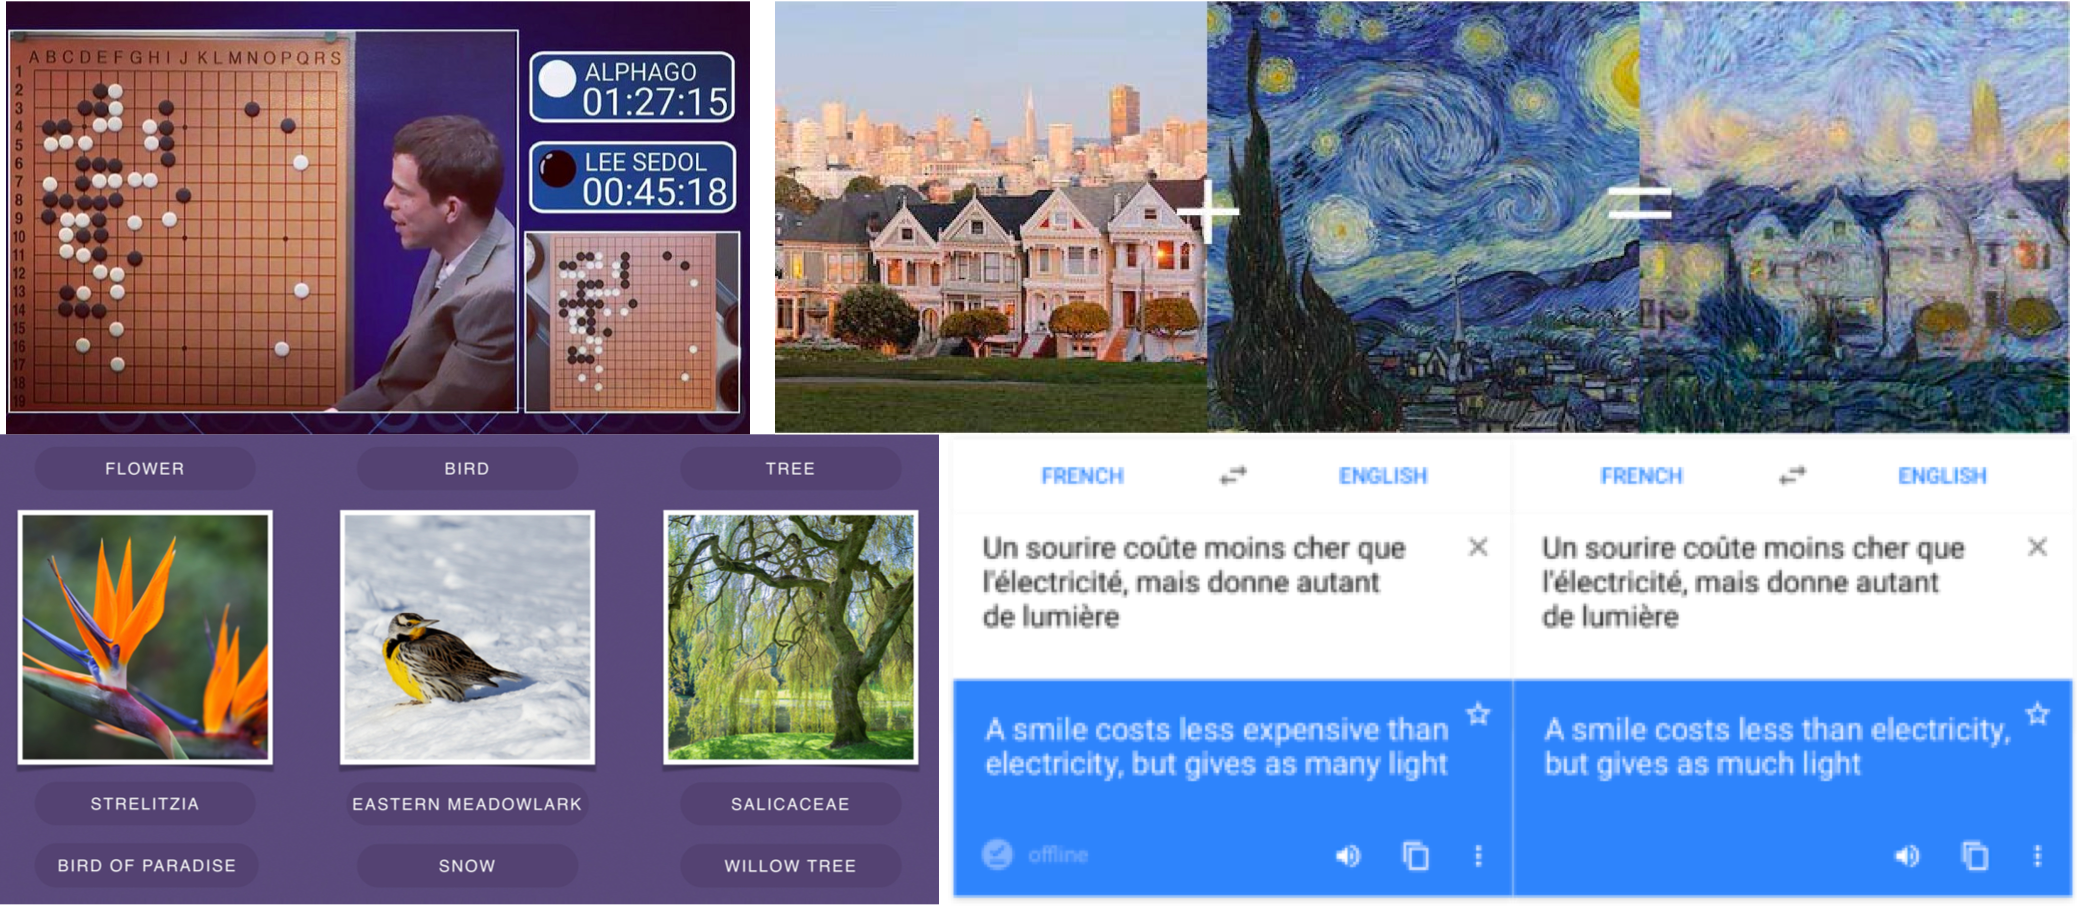
\includegraphics[width=.8\textwidth]{newstuff.png}
	\end{center}
Recent state-of-the-art results in \emph{game playing}, \emph{image recognition}, \emph{content generation}, \emph{natural language processing}, \emph{machine translation}, many other areas.  
\end{frame}

\begin{frame}
	\frametitle{modern neural networks}
	All changed with the introduction of AlexNet and the 2012 ImageNet Challenge...
	\begin{center}
		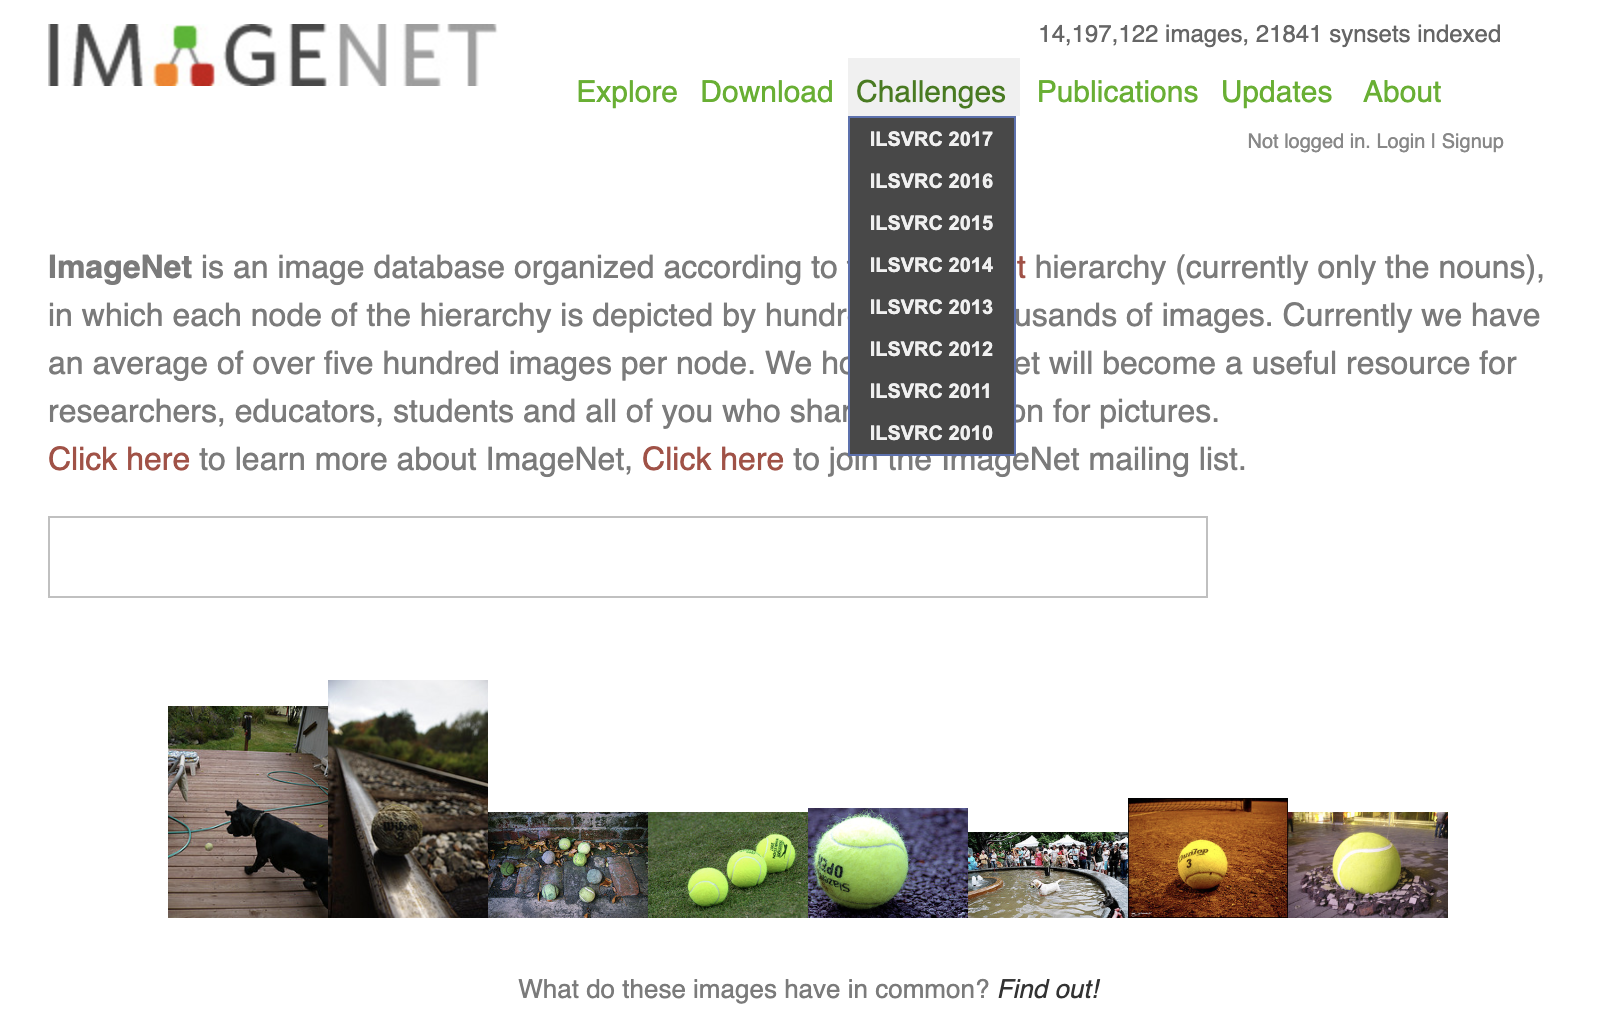
\includegraphics[width=.8\textwidth]{imagenet_page.png}
		
		Very general image classification task.
	\end{center}
\end{frame}

\begin{frame}
	\frametitle{modern neural networks}
	\small
	All changed with AlexNet and the 2012 ImageNet Challenge...
	\begin{center}
		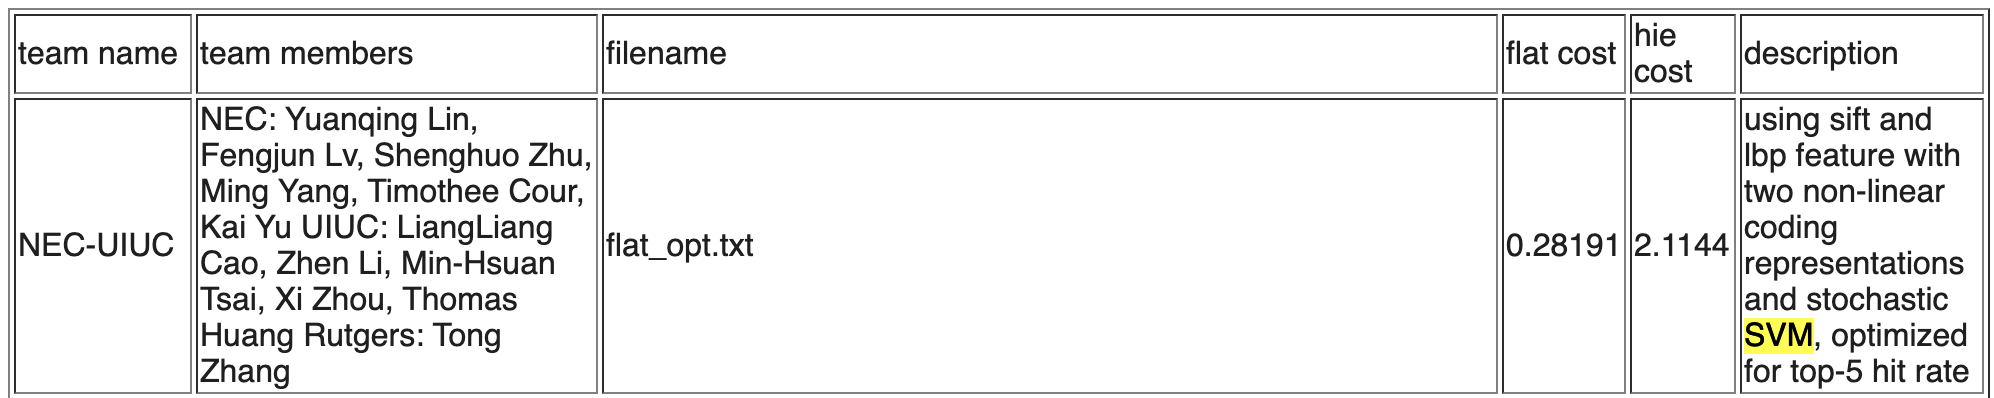
\includegraphics[width=.7\textwidth]{imagenet2010.png}
		
		2010 Results
	\end{center}
	\begin{center}
	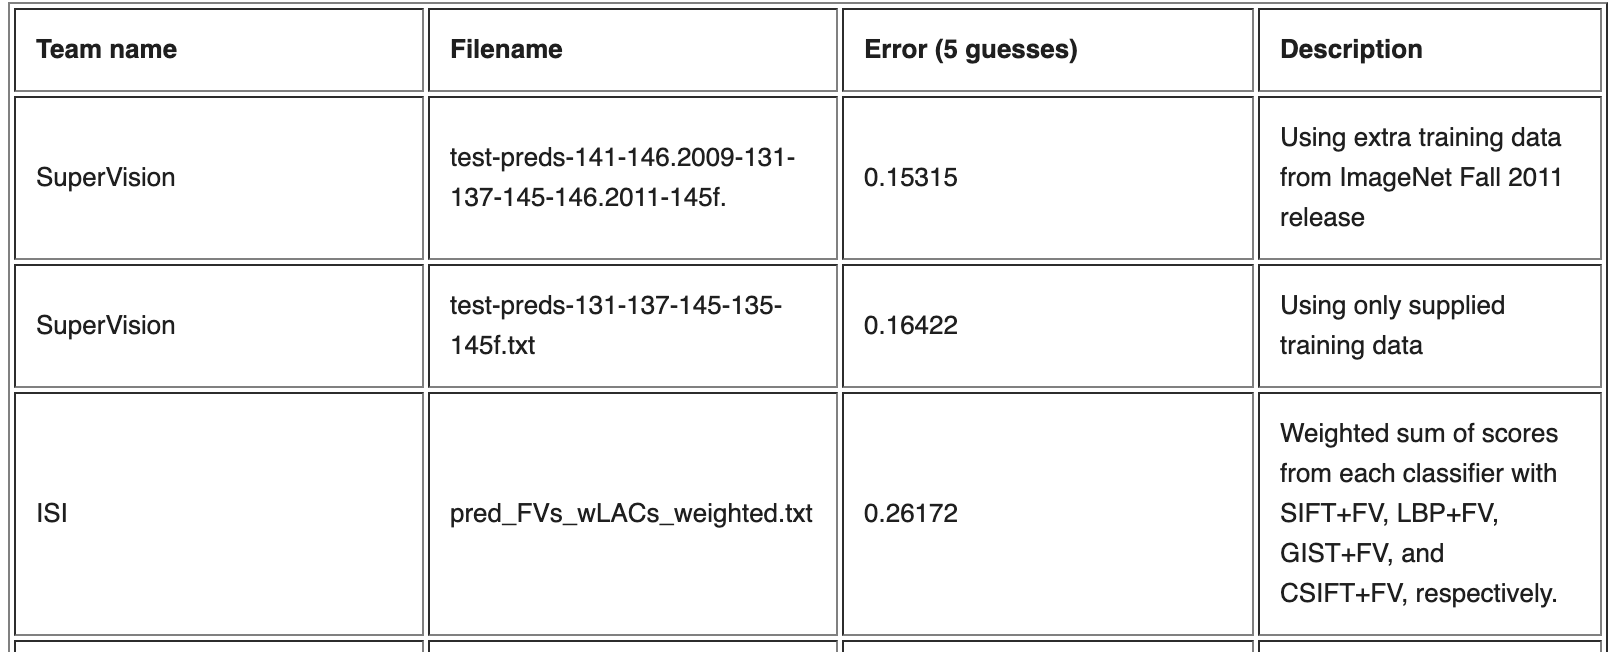
\includegraphics[width=.7\textwidth]{imagenet2012.png}
	
	2012 Results
	\end{center}
\end{frame}

\begin{frame}
	\frametitle{2019 turing award winners}
	\small
``For conceptual and engineering breakthroughs that have made deep neural networks a critical component of computing.''
		\begin{center}
		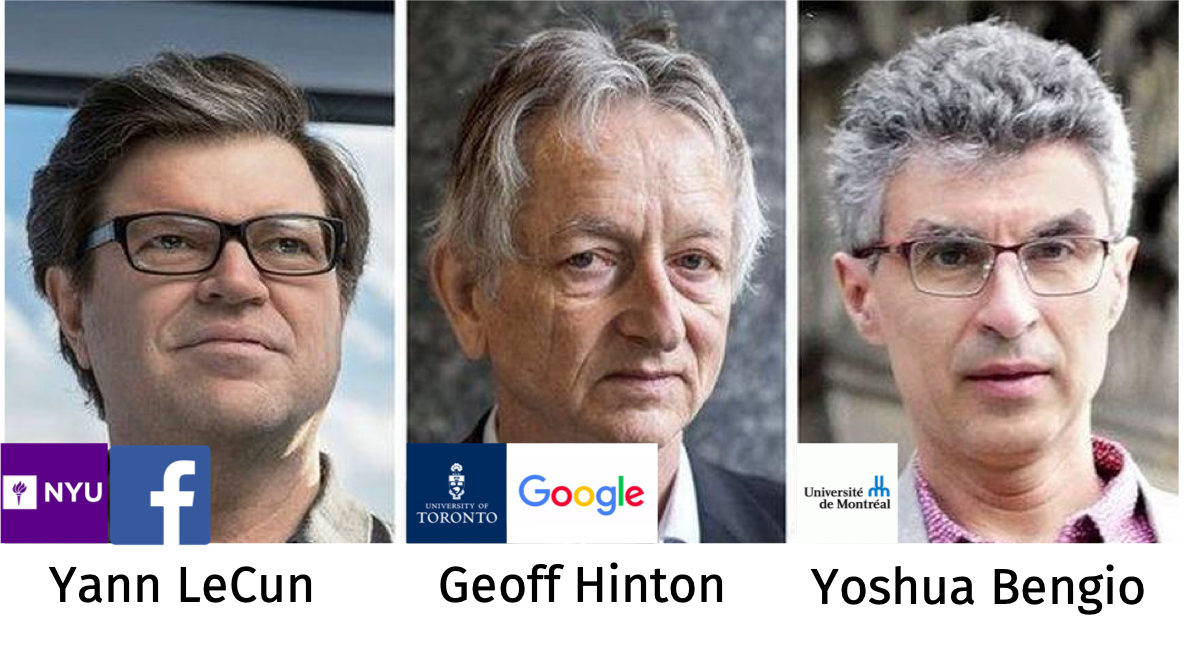
\includegraphics[width=.7\textwidth]{turing_annotate.png}
	\end{center}
	\textbf{What were these breakthroughs? What made training large neural networks computationally feasible?}
\end{frame}

\begin{frame}
	\frametitle{graphics processing unit}
	\textbf{Hardware innovation:} Widely available, inexpensive GPUs allowing for cheap, highly parallel linear algebra operations.
	
	\begin{itemize}
		\item 2007: Nvidia released CUDA platform, which allows GPUs to be easily programmed for general purposed computation.
	\end{itemize}
\begin{center}
	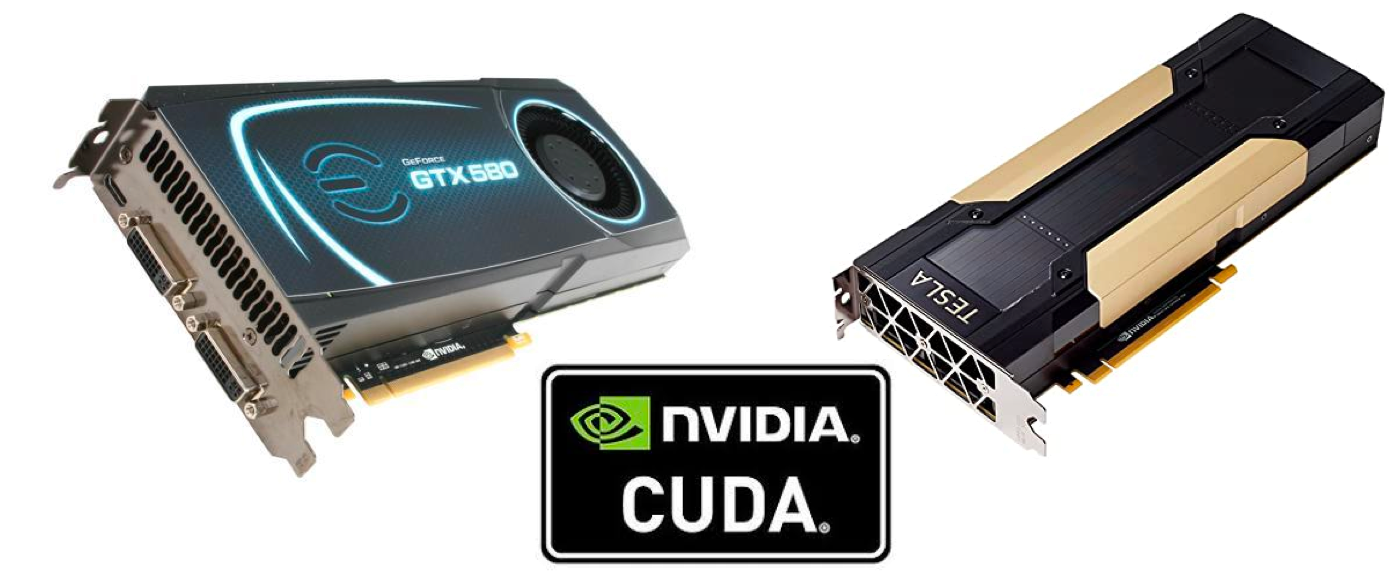
\includegraphics[width=.6\textwidth]{gpus.png}
\end{center}
AlexNet architecture used 60 million parameters. Could not have been trained using CPUs alone (except maybe on a government super computer).  
\end{frame}

\begin{frame}
	\frametitle{training neural networks}
	\textbf{Two main algorithmic tools for training neural network models:}
	\begin{enumerate}
		\item Stochastic gradient descent.
		\item Backpropogation.
	\end{enumerate}
\end{frame}

\begin{frame}
	\frametitle{training neural networks}
	Let $f(\vec{\theta},\vec{x})$ be our neural network. A typical $\ell$-layer feed forward model has the form:
	\begin{align*}
%	\bv{W}_\ell g\left(\ldots 
	g_{\ell}\left(\bv{W}_\ell\left(\ldots \bv{W}_3 \cdot g_2 \left(\bv{W}_2 \cdot g_1\left(\bv{W}_1\vec{x} + \vec{b}_1\right) + \vec{b}_2\right)+ \vec{b}_3 \ldots \right) + b_\ell\right).
	\end{align*} 
	$\bv{W}_{i}$ and $\vec{b}_i$ are the \emph{weight matrix} and \emph{bias vector} for layer $i$ and $g_i$ is the non-linearity (e.g. sigmoid). $\vec{\theta} = [\bv{W}_0,\vec{b}_0, \ldots,\bv{W}_\ell,\vec{b}_\ell]$ is a vector of all entries in these matrices.
	
	\textbf{Goal:} Given training data $(\vec{x}_1, y_1),\ldots,(\vec{x}_n, y_n)$ minimize the loss
	\begin{align*}
	\mathcal{L}(\vec{\theta}) = \sum_{i=1}^n L\left(y_i,f(\vec{\theta}, \vec{x}_i)\right)
	\end{align*}
	\textbf{Example:} We might use the binary cross-entropy loss for binary classification:
	\begin{align*}
		L\left(y_i,f(\vec{\theta}, \vec{x}_i)\right) = y_i\log(f(\vec{\theta},\vec{x}_i)) + (1-y_i)\log(1 - f(\vec{\theta}, \vec{x}_i))
	\end{align*}
\end{frame}

\begin{frame}
	\frametitle{gradient of the loss}
	\textbf{Most common approach:} minimize the loss by using \emph{gradient descent}. Which requires us to compute the gradient of the loss function, $\nabla \mathcal{L}$. Note that this gradient has an entry for \emph{every value} in $\bv{W}_0,\vec{b}_0, \ldots,\bv{W}_\ell,\vec{b}_\ell$.
	
	As usual, our loss function has \emph{finite sum} structure, so:
	\begin{align*}
	\nabla \mathcal{L}(\vec{\theta}) = \sum_{i=1}^n \nabla L\left(y_i,f(\vec{\theta},\vec{x}_i)\right)
	\end{align*}
	So we can focus on computing:
	\begin{align*}
	\nabla L\left(y,f(\vec{\theta},\vec{x})\right)
	\end{align*}
	for a single training example $(\vec{x}, y)$. 
\end{frame}

\begin{frame}[t]
	\frametitle{gradient of the loss}
	\textbf{Applying chain rule to loss:}
	\begin{align*}
		\nabla L\left(y,f(\vec{\theta},\vec{x})\right) = \frac{\partial L}{\partial f(\vec{\theta},\vec{x})}\cdot \nabla f(\vec{\theta},\vec{x})
	\end{align*}
	\textbf{Binary cross-entropy example:}
	\begin{align*}
	L\left(y,f(\vec{x})\right) = y\log(f(\vec{\theta},\vec{x})) + (1-y)\log(1 - f(\vec{\theta},\vec{x}))
	\end{align*}
\end{frame}

\begin{frame}
	\frametitle{gradient of the loss}
	We have reduced our goal to computing $\nabla f(\vec{\theta}, \vec{x})$, where the gradient is with respect to the parameters $\vec{\theta}$.
	
	\textbf{Back-propagation} is a natural and efficient way to compute $\nabla f(\vec{\theta}, \vec{x})$. It derives its name because we compute gradient from back to front: starting with the parameters closest to the output of the neural net.
\end{frame}

\begin{frame}
	\frametitle{backprop example}
	\small
	Let's understand how backprop works with a simple example.
	\vspace{-.5em}
	\begin{center}
		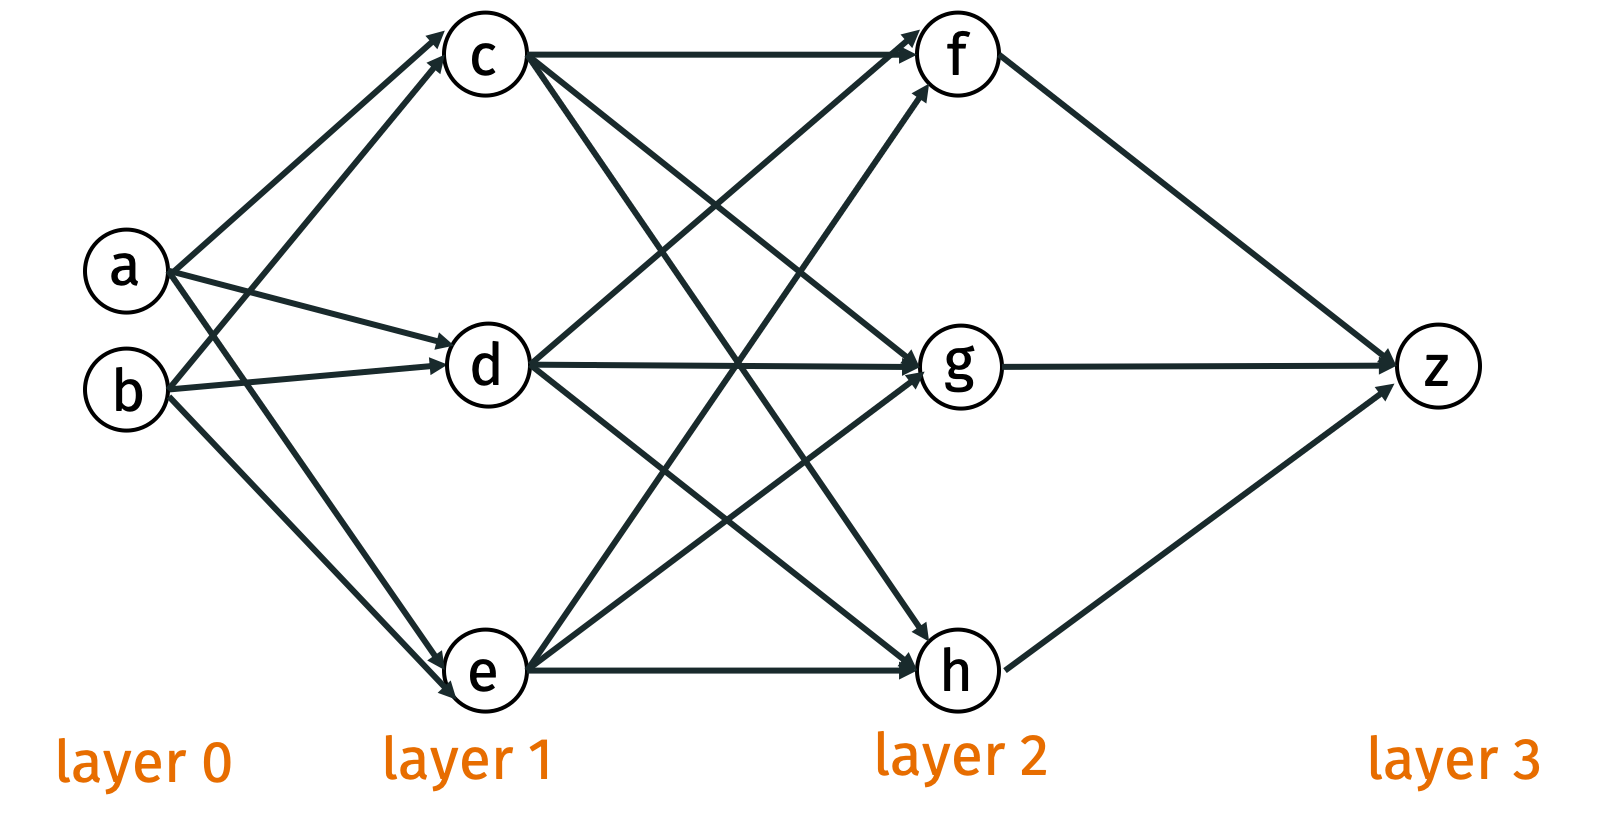
\includegraphics[width=.6\textwidth]{backpro_example.png}
		\vspace{-1em}
	\end{center}
Notation for next few slides:
\vspace{-1em}
\begin{itemize}
	\item $\vec{x} = [a,b]$. $f(\vec{\theta}, \vec{x}) = z$.
	\item $W_{i,j}$ is the weight of edge from node $i$ to node $j$. 
	\item $s(\cdot): \R\rightarrow \R$ is the non-linear activation function. 
	\item $b_{j}$ is the bias for node $j$.
\end{itemize}
	 \textbf{Example:} $h = s(c\cdot W_{c,h} + d\cdot W_{d,h} + e\cdot W_{e,h} + b_h)$
\end{frame}

\begin{frame}
	\frametitle{backprop example}
	For any node $j$, let $\bar{j}$ denote the value obtained \emph{before} applying the non-linearity $g$.
	\begin{center}
		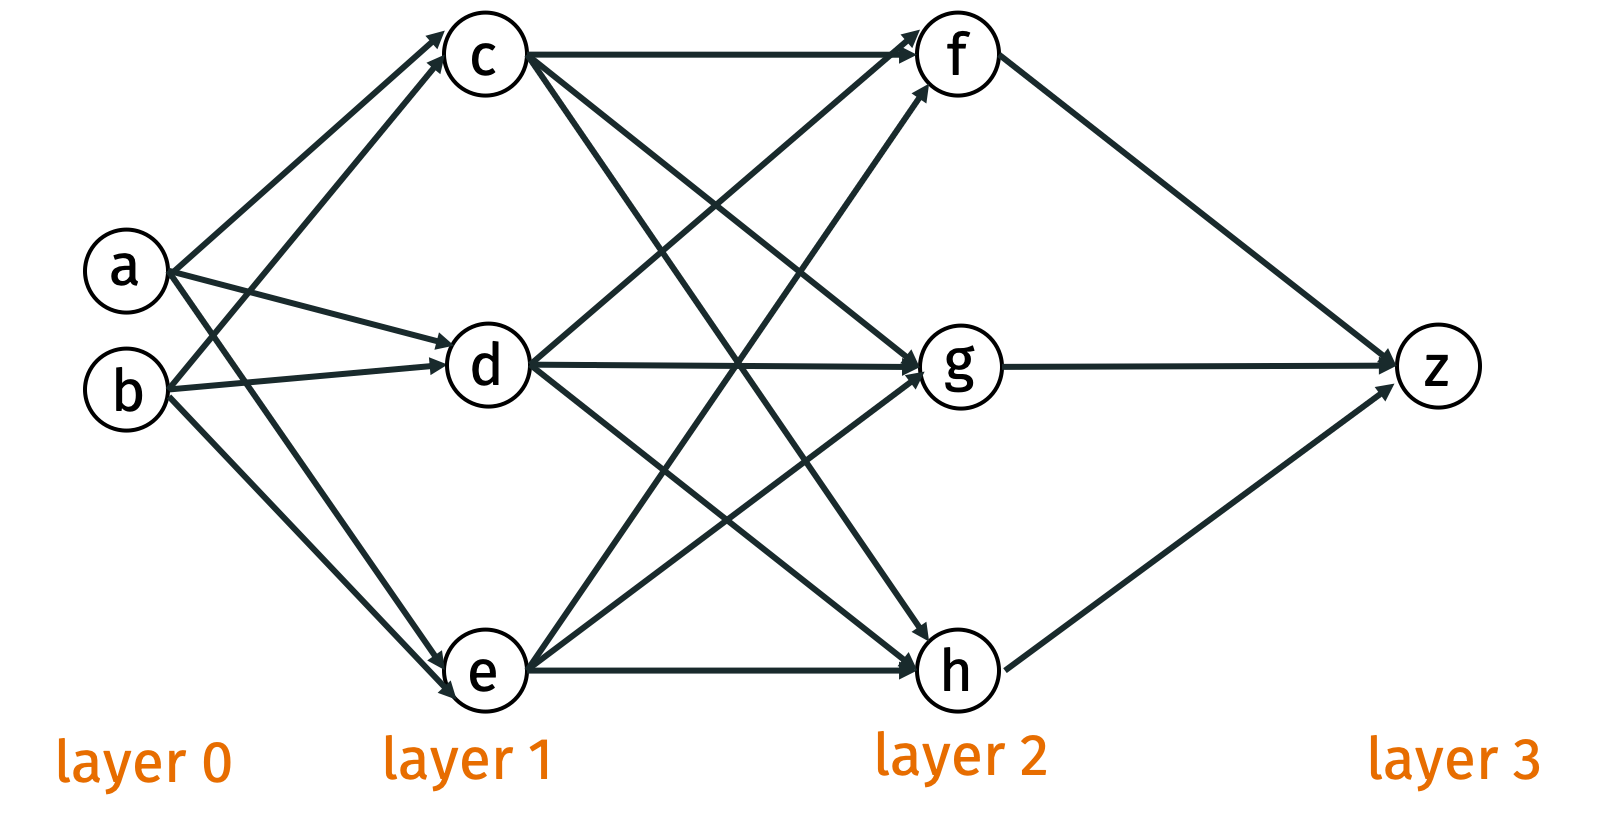
\includegraphics[width=.6\textwidth]{backpro_example.png}
		\vspace{-1em}
	\end{center}
So if $h = s(c\cdot W_{c,h} + d\cdot W_{d,h} + e\cdot W_{e,h} + b_h)$ then we use $\bar{h}$ to denote:
\begin{align*}
\bar{h} = c\cdot W_{c,h} + d\cdot W_{d,h} + e\cdot W_{e,h} + b_h
\end{align*}
\end{frame}

\begin{frame}
	\frametitle{backprop example}
	\textbf{Goal:} Compute the gradient $\nabla f(\vec{\theta},\vec{x})$, which contains the partial derivatives with respect to \emph{every} parameter:
	\begin{itemize}
		\item $\partial z / \partial b_z$
		\item $\partial z / \partial W_{f,z}$, $\partial z / \partial W_{g,z}$, $\partial z / \partial W_{h,z}$
		\item $\partial z / \partial b_f$, $\partial z / \partial  b_g$, $\partial z / \partial b_h$
		\item $\partial z / \partial W_{c,f}$, $\partial z / \partial W_{c,g}$, $\partial z / \partial W_{c,h}$
		\item $\partial z / \partial W_{d,f}$, $\partial z / \partial W_{d,g}$, $\partial z / \partial W_{d,h}$
		\item $\vdots$
		\item $\partial z / \partial W_{a,c}$, $\partial z / \partial W_{a,d}$, $\partial z / \partial W_{a,e}$
	\end{itemize}
\textbf{Two steps:} \emph{Forward pass} to compute function value. \emph{Backwards pass} to compute gradients. 
\end{frame}

\begin{frame}
	\frametitle{backprop example}
	\textbf{Step 1:} Forward pass. 
	\begin{center}
		\vspace{-.5em}
		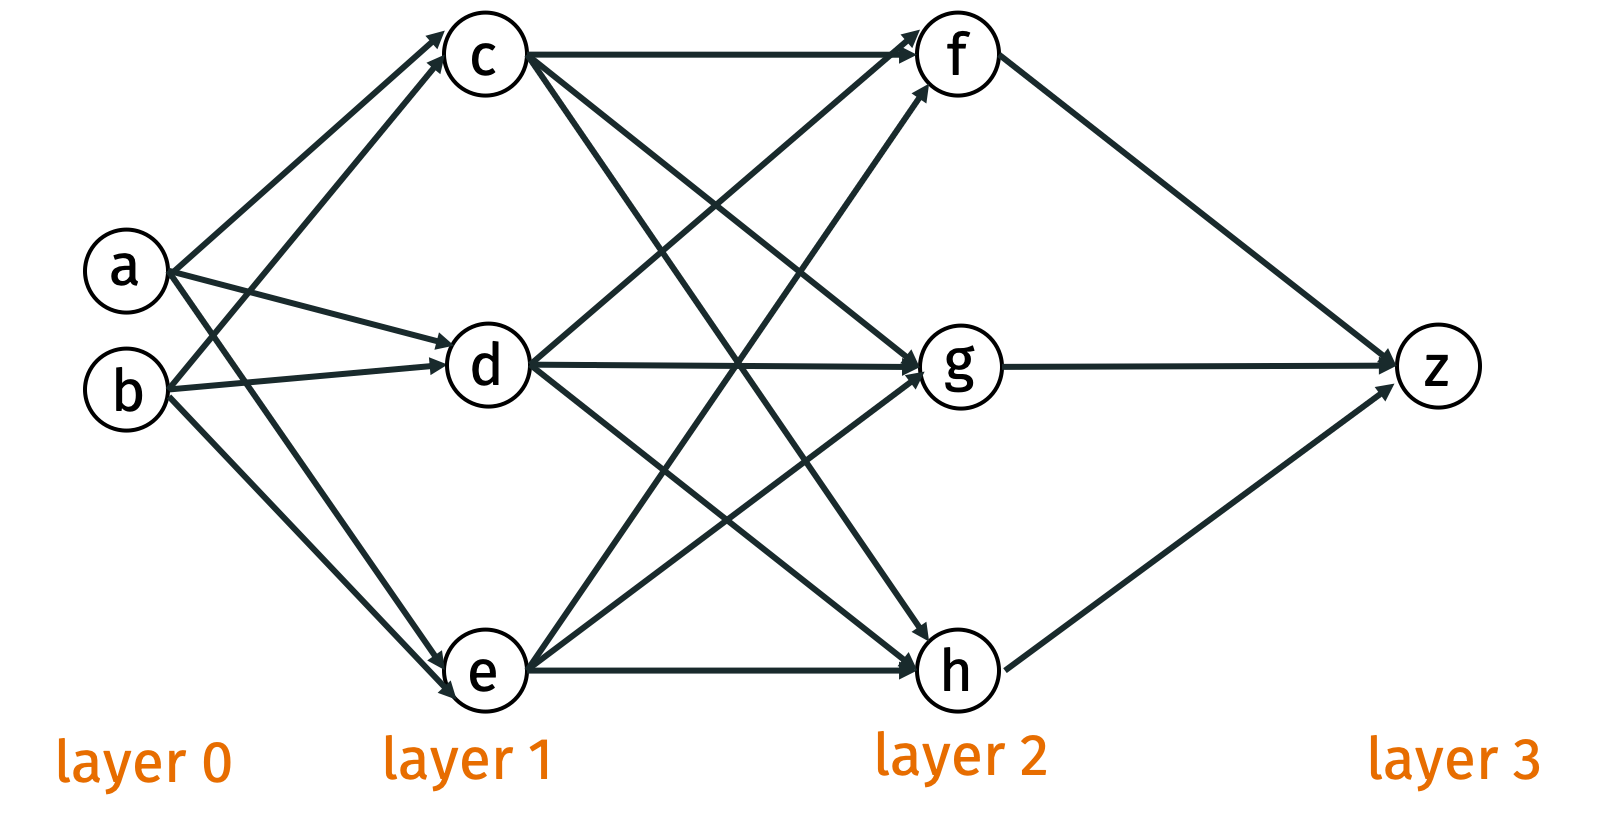
\includegraphics[width=.6\textwidth]{backpro_example.png}
		\vspace{-1em}
	\end{center}
\begin{itemize}
	\item Using current parameters, compute the output $z$ by moving from left to right.
	\item Store all intermediate results: \begin{align*}\bar{c}, \bar{d}, \bar{e}, c,d,e, \bar{f}, \bar{g}, \bar{h}, f,g,h, \bar{z}, z. \end{align*}
\end{itemize}	
\end{frame}

\begin{frame}[t]
	\frametitle{backprop example}
	\textbf{Step 1:} Forward pass. 
	
		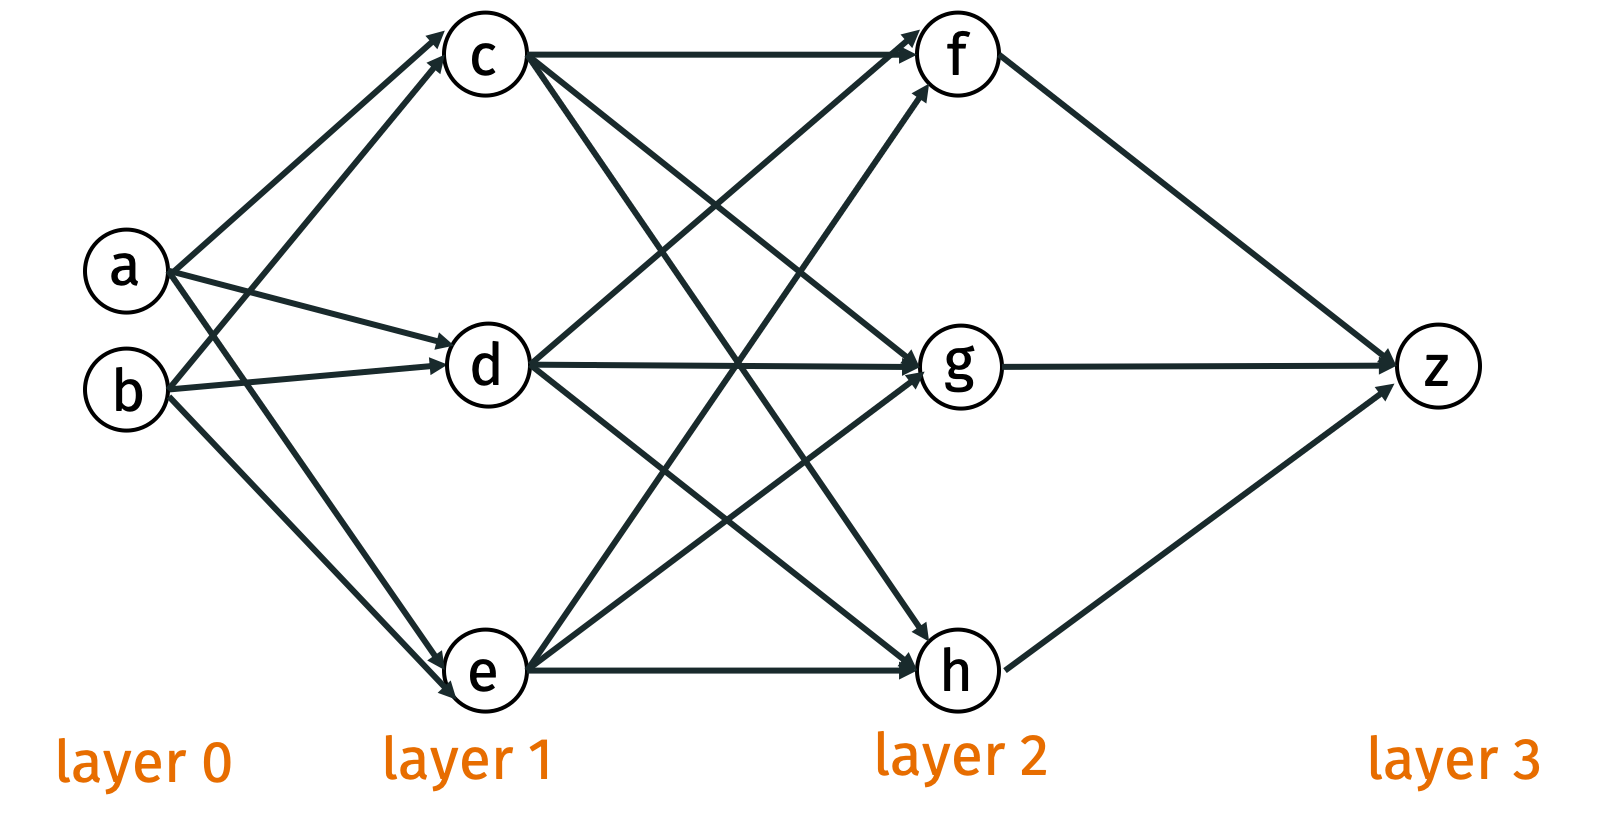
\includegraphics[width=.5\textwidth]{backpro_example.png}
\end{frame}

\begin{frame}
	\frametitle{backprop example}
	\textbf{Step 2:} Backward pass. 
	\begin{center}
		\vspace{-.5em}
		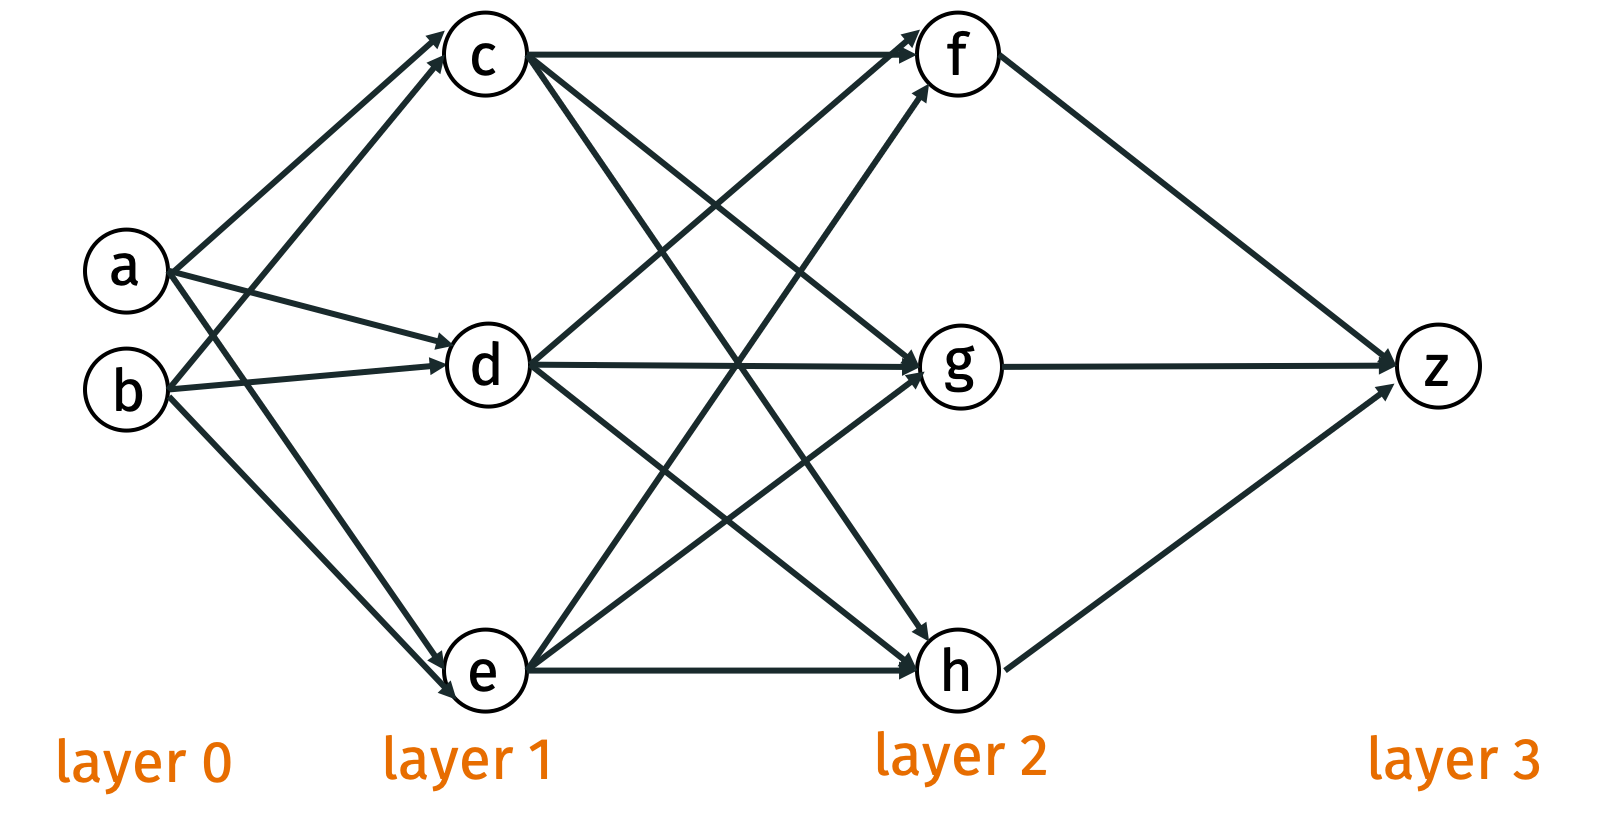
\includegraphics[width=.6\textwidth]{backpro_example.png}
		\vspace{-1em}
	\end{center}
	\begin{itemize}
		\item Using current parameters and computed node values, compute the partial derivatives of all parameters by moving from \emph{right to left}.
	\end{itemize}	
\end{frame}

\begin{frame}[t]
	\frametitle{backprop example}
	\textbf{Step 2:} Backward pass.  
	
	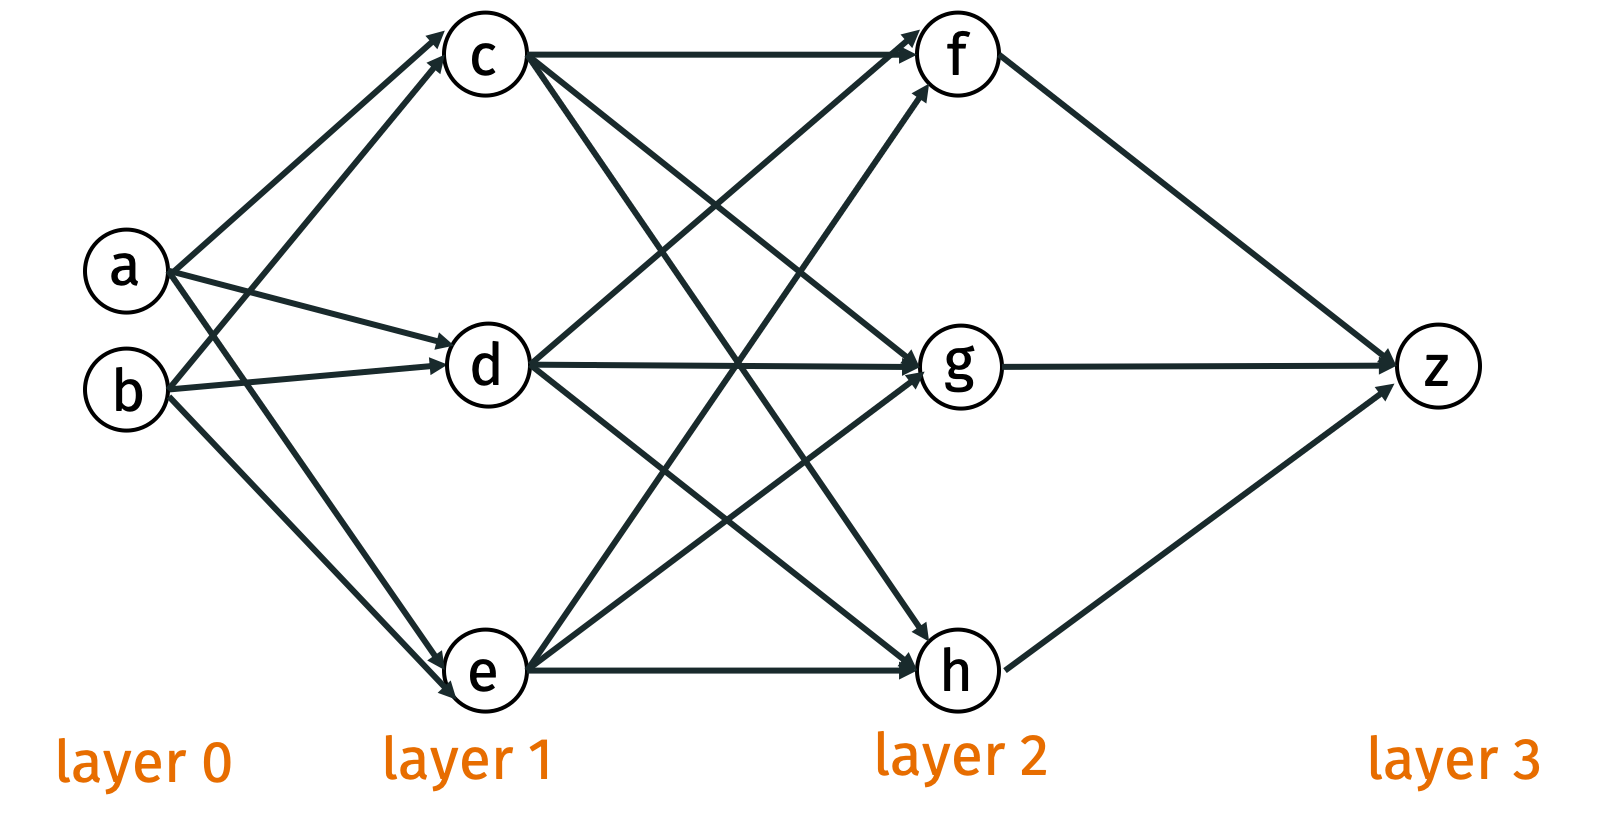
\includegraphics[width=.5\textwidth]{backpro_example.png}
\end{frame}

\begin{frame}[t]
	\frametitle{backprop example}
	\textbf{Step 2:} Backward pass.  
	
	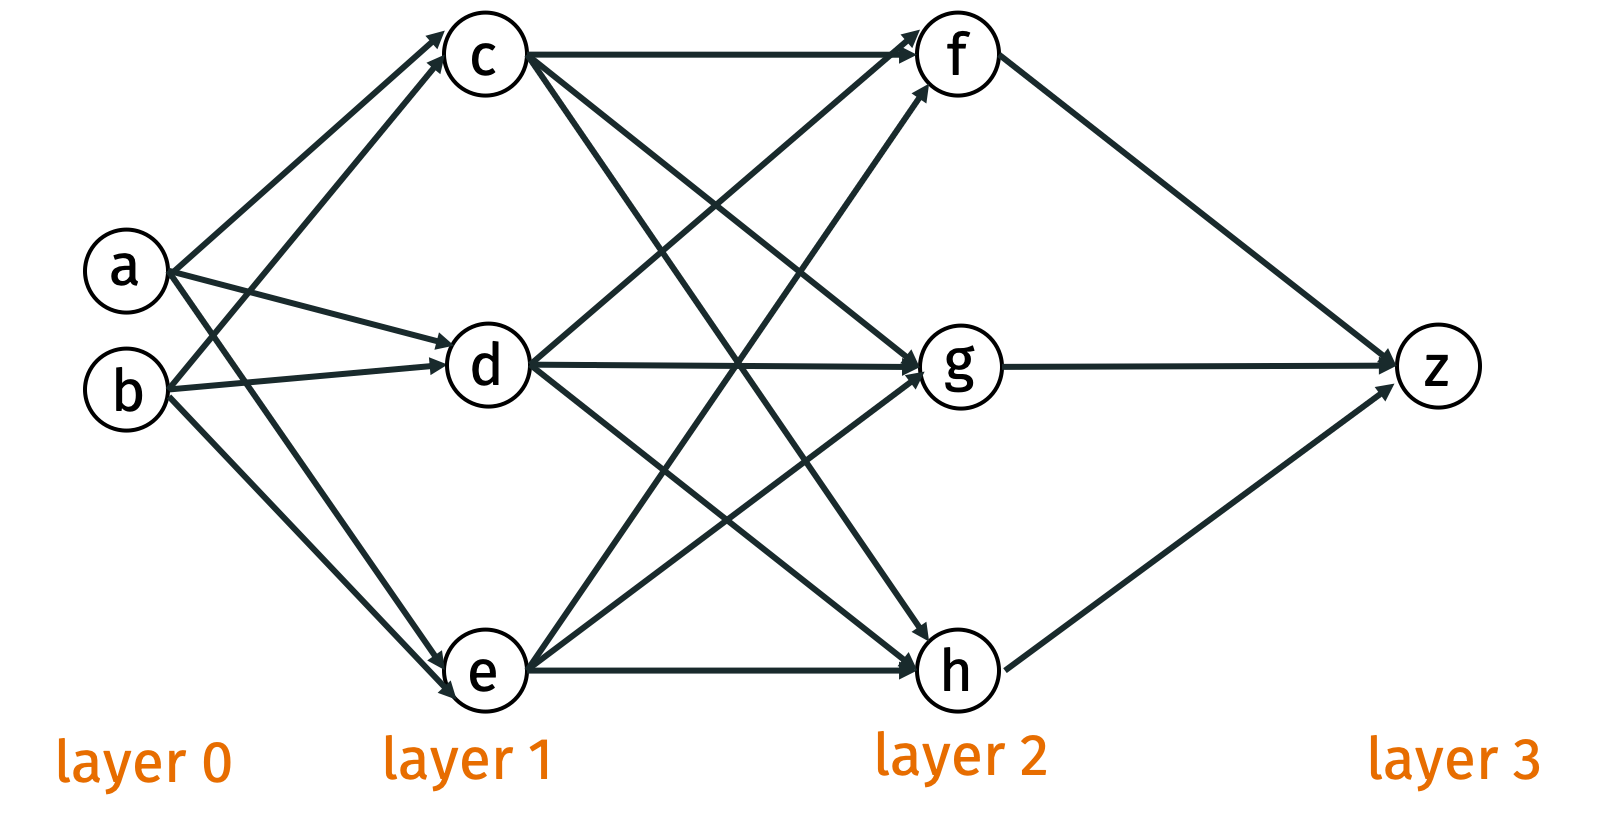
\includegraphics[width=.5\textwidth]{backpro_example.png}
\end{frame}

\begin{frame}
	\frametitle{backprop linear algebra}
	\small
	\textbf{Linear algebraic view}. 
	
	Let $\vec{\delta}_i$ be a vector containing $\partial z /\partial j$ for all nodes $j$ in layer $i$. 
	\begin{align*}
	\delta_3 &= \begin{bmatrix}1\end{bmatrix} & \vec{\delta}_2 &= \begin{bmatrix}\partial z /\partial f\\\partial z /\partial g\\\partial z /\partial h\end{bmatrix} & \vec{\delta}_1 &= \begin{bmatrix}\partial z /\partial c\\\partial z /\partial d\\\partial z /\partial e\end{bmatrix} 
	\end{align*}
	Let $\bar{\delta}_i$ be a vector containing $\partial z /\partial \bar{j}$ for all nodes $j$ in layer $i$. 
	\begin{align*}
	\bar{\delta}_3 &= \begin{bmatrix}\partial z /\partial \bar{z}\end{bmatrix} & \delta_2 &= \begin{bmatrix}\partial z /\partial \bar{f}\\\partial z /\partial \bar{g}\\\partial z /\partial \bar{h}\end{bmatrix} & \bar{\delta}_1 &= \begin{bmatrix}\partial z /\partial \bar{c}\\\partial z /\partial \bar{d}\\ \partial z /\partial \bar{e}\end{bmatrix} 
	\end{align*}
	
	\textbf{Note:} $\bar{\delta}_i = s'(\vec{\delta}_i) \times \vec{\delta}_i$ where $s'$ is the derivative $s'$ and this function, as well as the $\times$ are applied entrywise. 
\end{frame}

\begin{frame}
	\frametitle{backprop linear algebra}
	\small
	 
	Let $\bv{W}_i$ be a matrix containing all the weights for edges between layer $i$ and layer $i+1$. 
	
	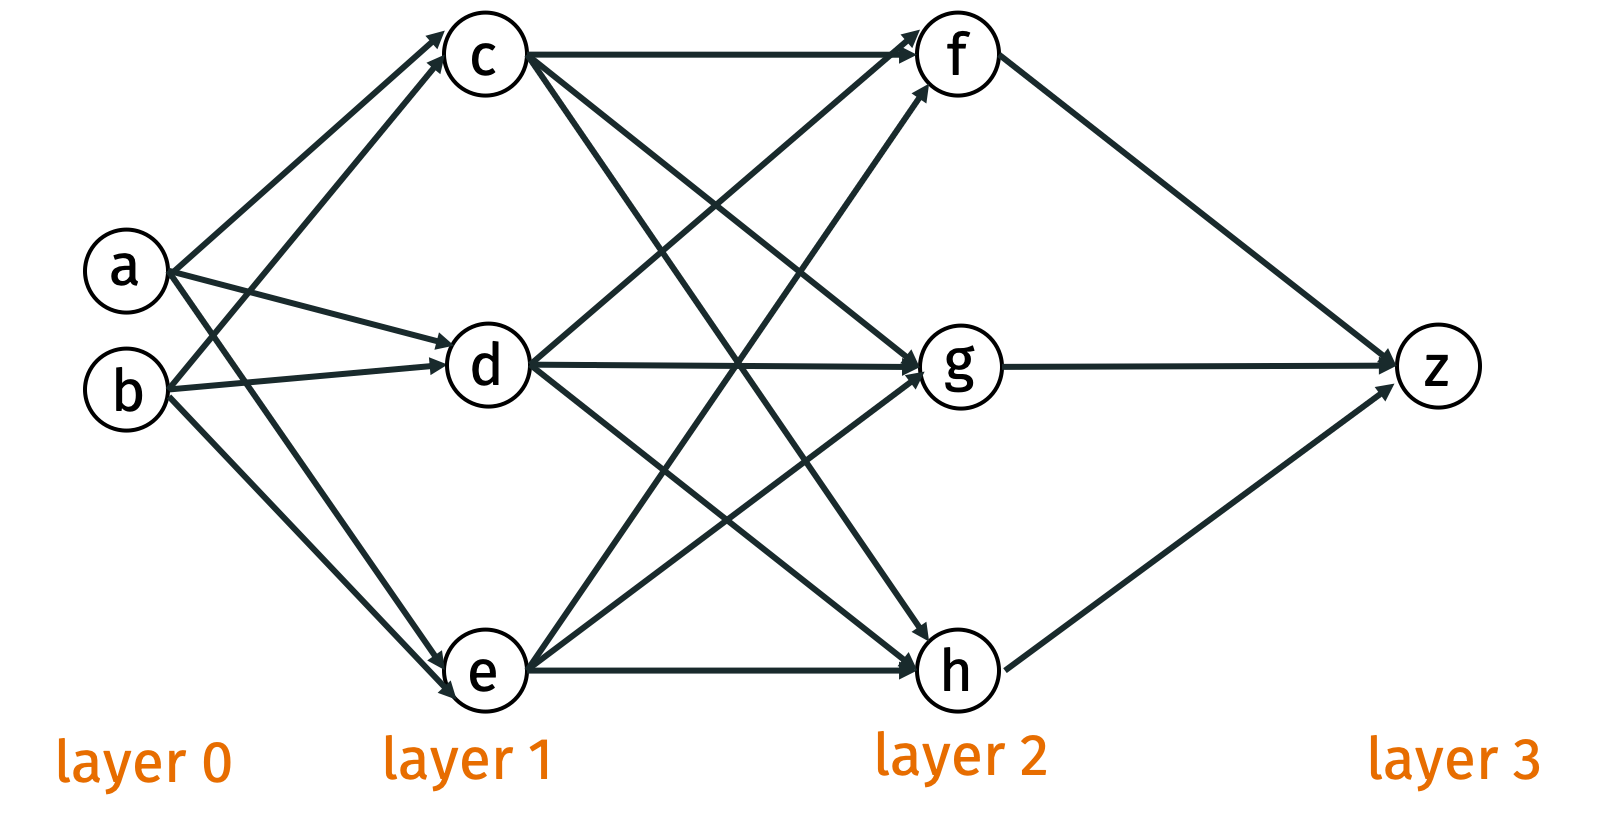
\includegraphics[width=.5\textwidth]{backpro_example.png}
	\begin{align*}
	\bv{W}_2 &= \begin{bmatrix}W_{f,z}&W_{g,z}& W_{h,z}\end{bmatrix} & \bv{W}_1 &= \begin{bmatrix}W_{c,f}&W_{d,f}& W_{e,f}\\
	W_{c,g}&W_{d,g}& W_{e,g}\\
	W_{c,h}&W_{d,h}& W_{e,h}
	\end{bmatrix}
	& \bv{W}_0 &= \begin{bmatrix}W_{a,c}&W_{b,c}\\
	W_{a,d}&W_{b,d}\\
	W_{a,e}&W_{b,e}
	\end{bmatrix}
	\end{align*}
\end{frame}

\begin{frame}
	\frametitle{backprop linear algebra}
	\small
	
	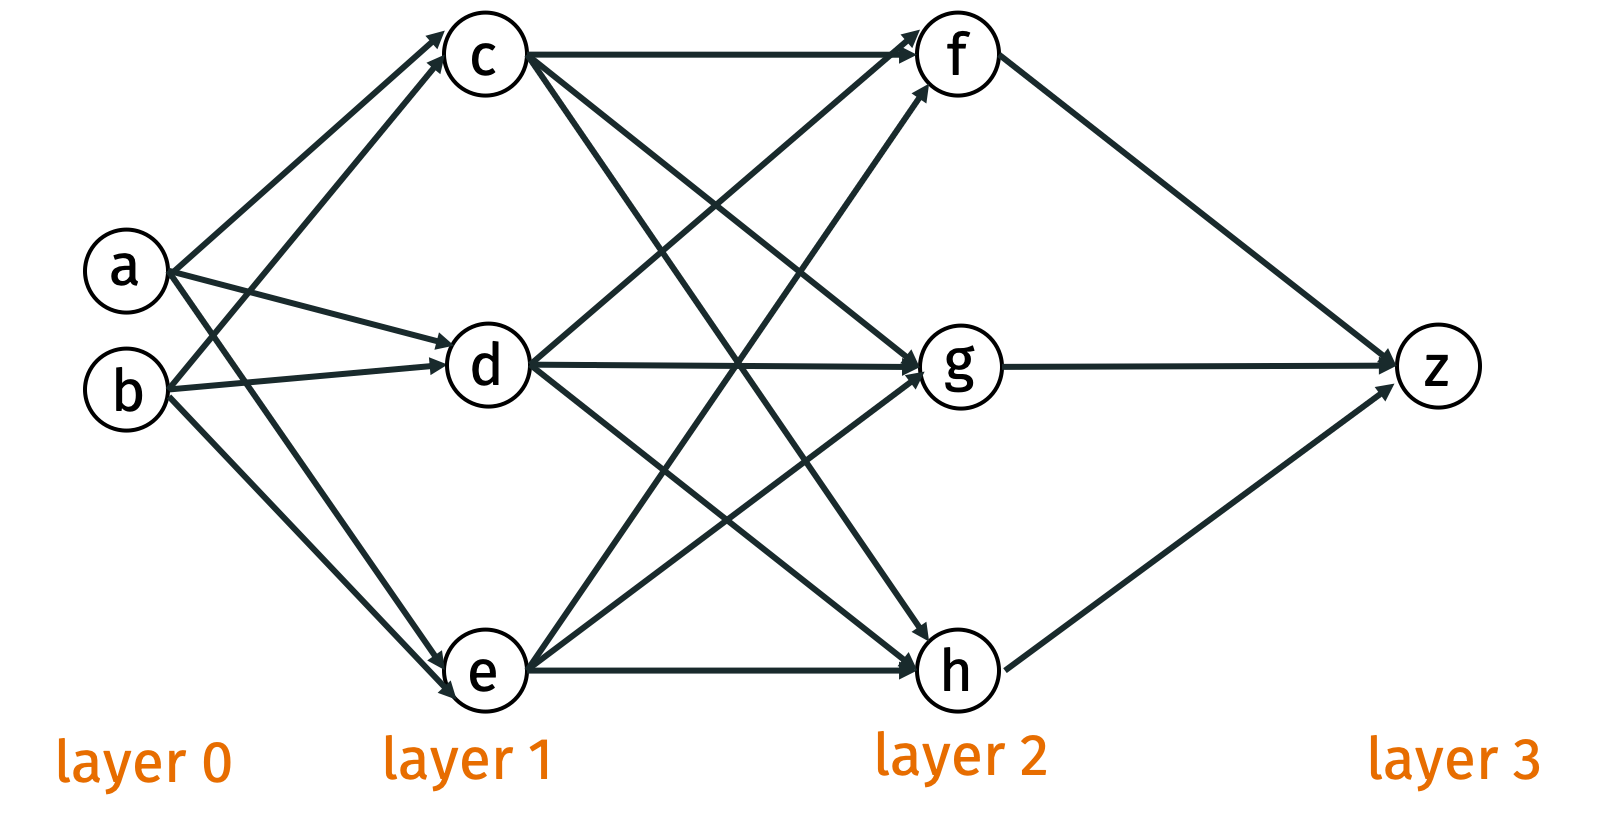
\includegraphics[width=.5\textwidth]{backpro_example.png}

	\textbf{Claim 1:} Node derivative computation is matrix multiplication.
	\begin{align*}
		\vec{\delta}_i = \bv{W}_i^T \bar{\delta}_{i+1}
	\end{align*}
\end{frame}

\begin{frame}
	\frametitle{backprop linear algebra}
	\small
	
	Let $\bs{\Delta}_i$ be a matrix contain the derivatives for all weights for edges between layer $i$ and layer $i+1$. 
	
	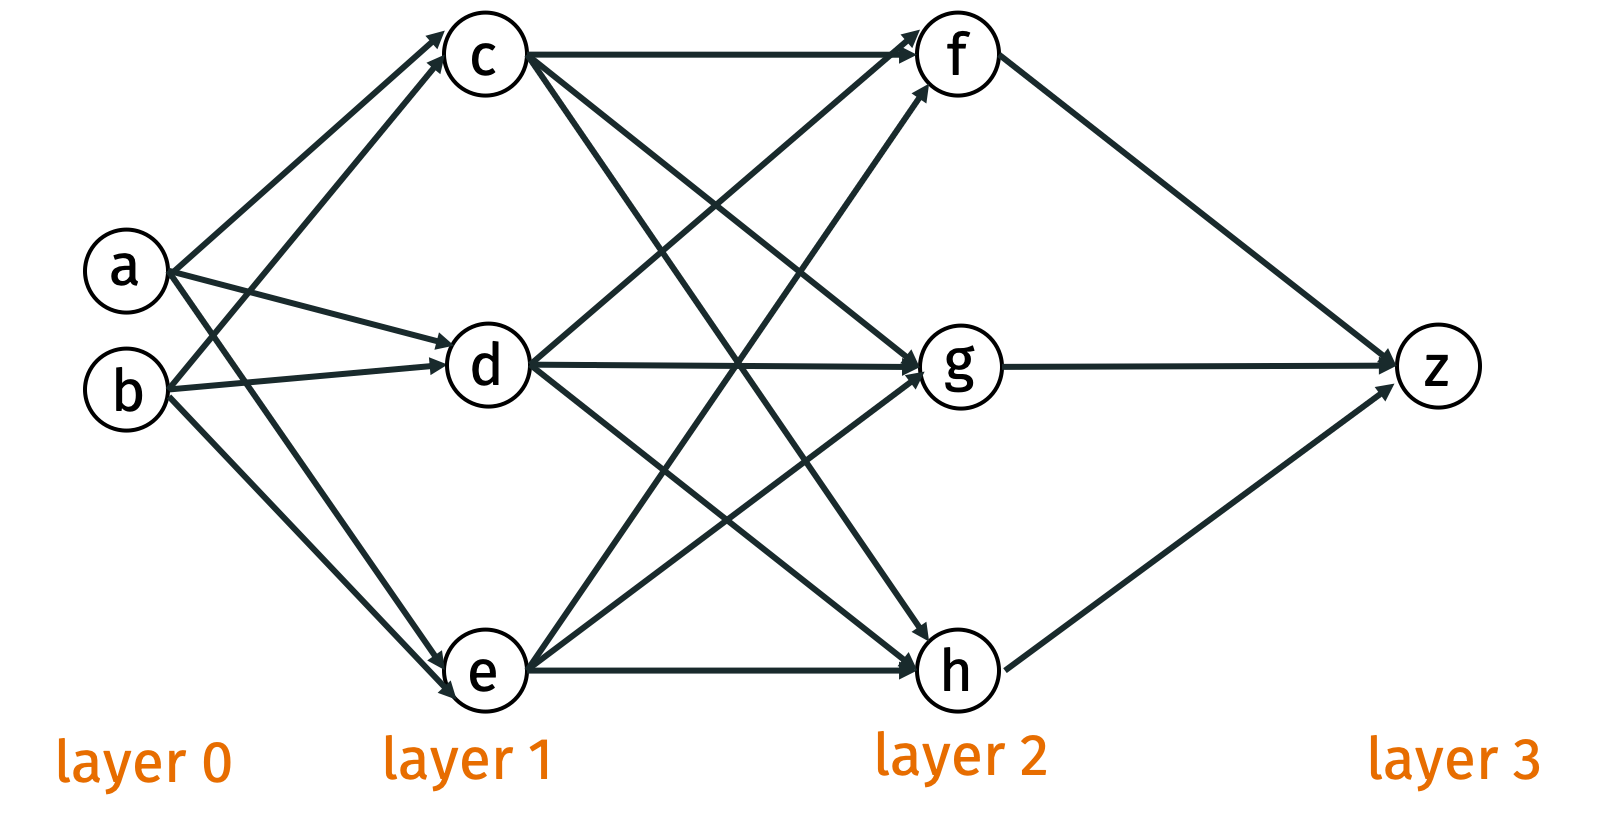
\includegraphics[width=.5\textwidth]{backpro_example.png}
	\begin{align*}
\bs{\Delta}_2 &= \begin{bmatrix}\partial z/\partial W_{f,z}&\partial z/\partial W_{g,z}& \partial z/\partial W_{h,z}\end{bmatrix} \\
\bs{\Delta}_1 &= \begin{bmatrix}\partial z/\partial W_{c,f}&\partial z/\partial W_{d,f}& \partial z/\partial W_{e,f}\\
\partial z/\partial W_{c,g}&\partial z/\partial W_{d,g}& \partial z/\partial W_{e,g}\\
\partial z/\partial W_{c,h}&\partial z/\partial W_{d,h}& \partial z/\partial W_{e,h}
\end{bmatrix}\\
\bs{\Delta}_0 &= \ldots
\end{align*}
\end{frame}

\begin{frame}
\frametitle{backprop linear algebra}
	\small
	
	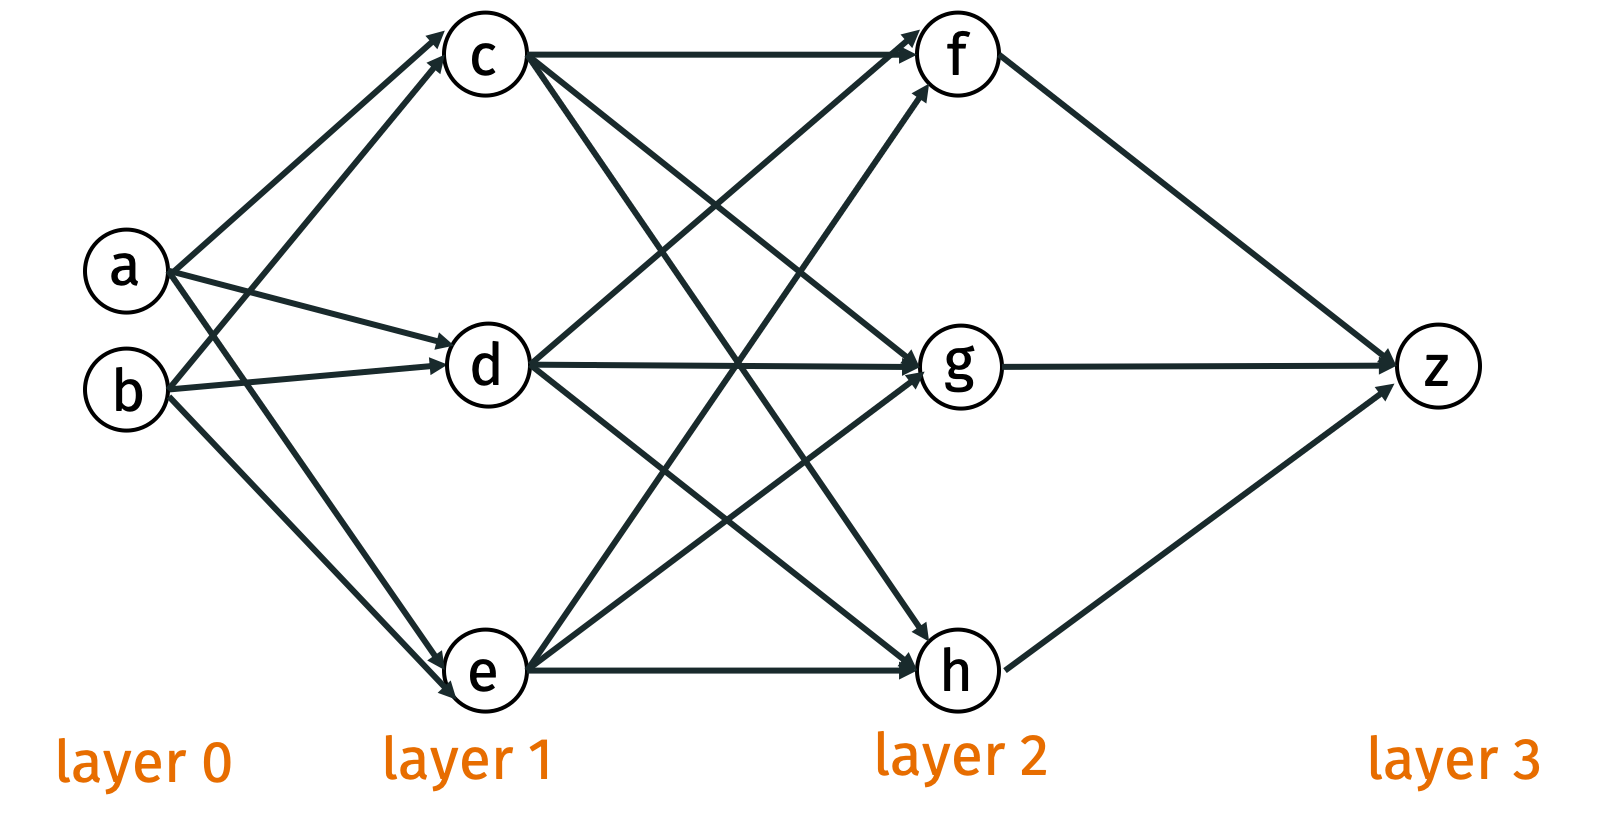
\includegraphics[width=.5\textwidth]{backpro_example.png}
	
	\textbf{Claim 2:} Weight derivative computation is an outer-product.
	\begin{align*}
	\bs{\Delta}_i = \vec{v}_i\bar{\delta}_{i+1}^T
	\end{align*}
	where $\vec{v}_i$ contains the values of all nodes in layer $i$. E.g. $\vec{v}_0 = \begin{bmatrix}
	a\\b
	\end{bmatrix}$. 
\end{frame}

\begin{frame}
	\frametitle{backprop example}
	\textbf{Takeaways:}
	\begin{itemize}
		\item Backpropogation can be used to compute derivatives for all weights and biases for any feedforward neural network.
		\item Final computation boils down to linear algebra operations (matrix multiplication and vector operations) which can be performed quickly on a GPU.
	\end{itemize}

We computed $\nabla L\left(y_i,f(\vec{\theta}, \vec{x}_i)\right)$ for a \emph{single training example} $(\vec{x}_i, y_i)$. Computing entire gradient requires computing:
	\begin{align*}
\nabla \mathcal{L}(\vec{\theta}) = \sum_{i=1}^n \nabla L\left(y_i,f(\vec{\theta},\vec{x}_i)\right)
\end{align*}
\begin{center}
	\textbf{Computing the entire sum would be very expensive.}
\end{center}
\end{frame}

\begin{frame}
	\frametitle{training neural networks}
	\textbf{Second tool:} Stochastic Gradient Descent (SGD).
	\begin{itemize}
		\item Powerful {randomized} variant of GD used to train neural networks (or any other model where \emph{computing gradients is expensive}.
	\end{itemize}
\vspace{2em}
	\textbf{Recall gradient descent update:}
	\begin{itemize}
		\item For $t = 1, \ldots, T$:
		\begin{itemize}
		\item $\vec{\theta}_{t+1} = \vec{\theta}_{t} - \eta \nabla \mathcal{L}(\vec{\theta}_t)$
		\end{itemize}
	\end{itemize}
where $\eta$ is a learning rate parameter. 
\end{frame}

\begin{frame}
	\frametitle{stochastic gradient descent}
	Let $L_j(\vec{\theta})$ denote $L\left(y_j,f(\vec{\theta},\vec{x}_j)\right)$.
	
	\textbf{Claim:} If $j \in 1, \ldots, n$ is chosen uniformly at random. Then:
	\begin{align*}
	n\cdot\E\left[\nabla L_j(\vec{\theta}) \right] = \nabla \mathcal{L}(\vec{\theta}).
	\end{align*}
	\vspace{5em}
	
	$\nabla L_j(\vec{\theta})$ is called a \textbf{\alert{stochastic gradient}}.
\end{frame}

\begin{frame}
	\frametitle{stochastic gradient descent}
	\textbf{SGD iteration:}
	\begin{itemize}
		\item Initialize $\vec{\theta}_0$ (typically randomly).
		\item For $t = 1, \ldots, T$:
		\begin{itemize}
			\item Choose $j$ uniformly at random.
			\item Compute stochastic gradient $\vec{g} = \nabla L_j(\vec{\theta_t})$.
			\begin{itemize}
				\item For neural networks this is done using backprop with training example $(\vec{x}_j, y_j)$. 
			\end{itemize}
			\item Update $\vec{\theta}_{t+1} = \vec{\theta}_{t} - \eta \vec{g}$
		\end{itemize}
	\end{itemize}
\begin{center}
	\textbf{\alert{Move in direction of steepest descent \emph{in expectation.}}}
\end{center}
\end{frame}

\begin{frame}
	\frametitle{stochastic gradient descent}
	\textbf{Gradient descent:} Fewer iterations to converge, higher cost per iteration.
	
	\textbf{Stochastic Gradient descent:} More iterations to converge, lower cost per iteration.
	
	\begin{center}
		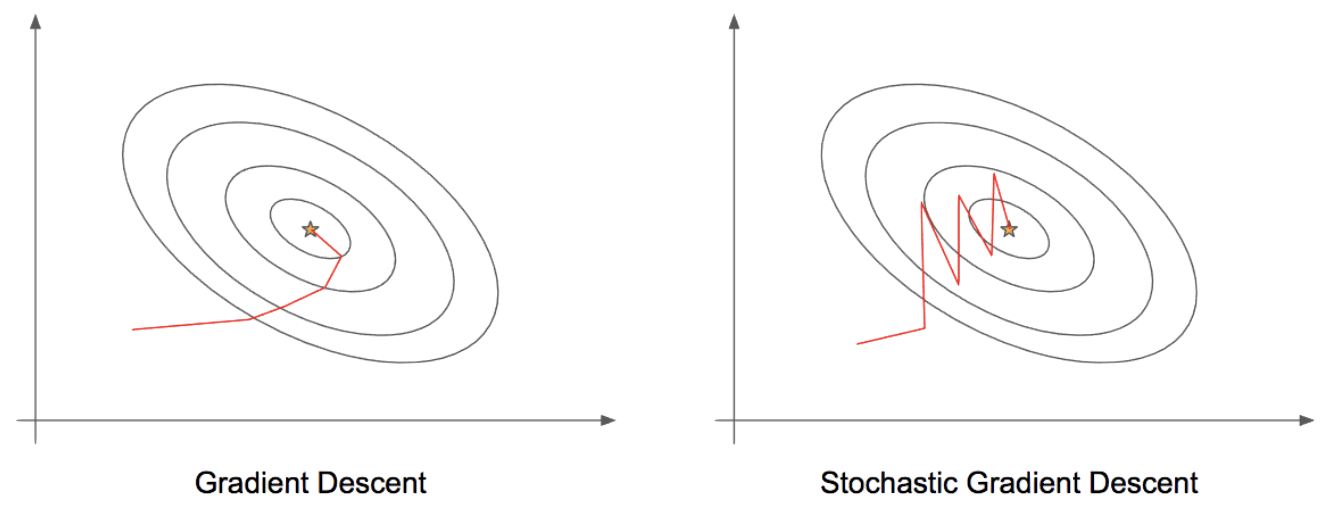
\includegraphics[width=\textwidth]{sgd_path_tame.png}
	\end{center}
\end{frame}

\begin{frame}
	\frametitle{stochastic gradient descent}
	\textbf{Gradient descent:} Fewer iterations to converge, higher cost per iteration.
	
	\textbf{Stochastic Gradient descent:} More iterations to converge, lower cost per iteration.
	
	\begin{center}
		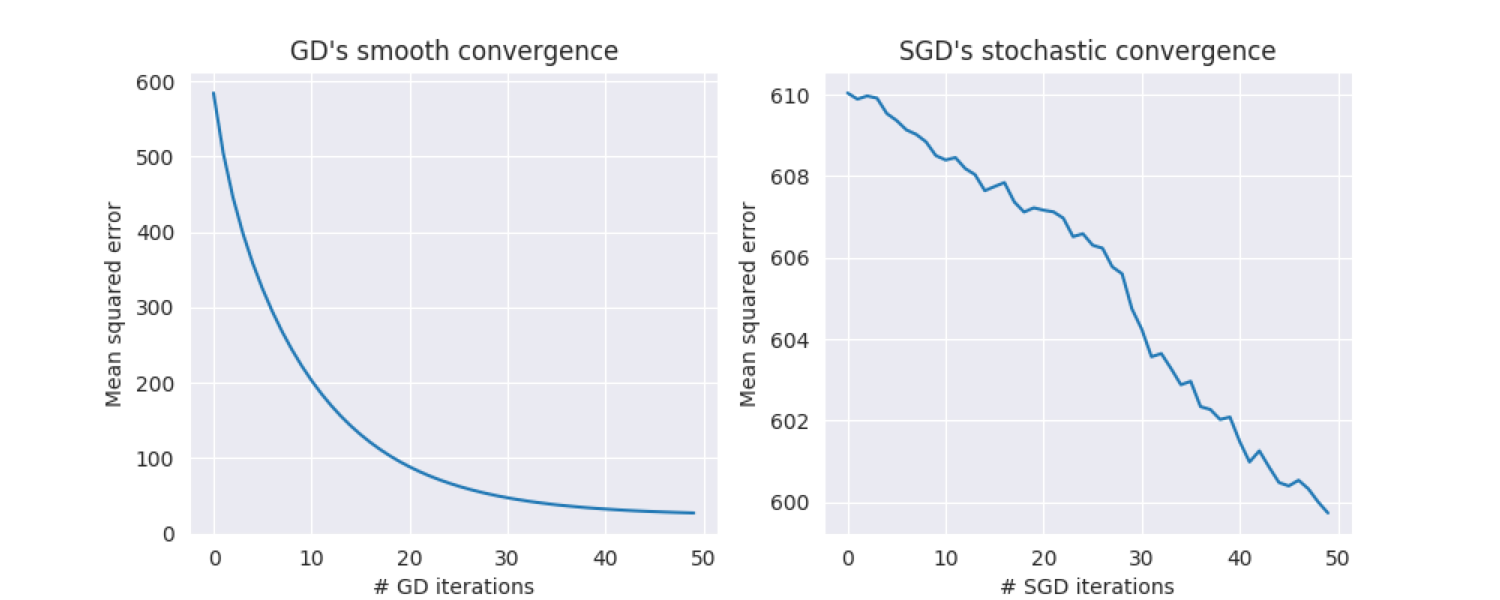
\includegraphics[width=.9\textwidth]{gd_convergence.png}
	\end{center}
\end{frame}

\begin{frame}
	\frametitle{stochastic gradient descent in practice}
	\emph{Practical Modification 1: \textbf{Cyclic Gradient Descent.}}
	
	Assume order of data is relatively random. Instead of choosing $j$ randomly at each iteration, choose $j = 1, j = 2, \ldots, j = n, j= 1, \ldots, j=n, \ldots$.  
	
	\textbf{Question:} Why might we want to do this?
	
\vspace{4em}
\begin{itemize}
	\item Relatively similar convergence behavior to standard SGD. 
	\item \textbf{Import term:} one \alert{\textbf{epoch}} denotes one pass over all training examples: $j= 1, \ldots, j=n$. 
	\item Convergence rates for training neural networks are often discussed in terms of epochs instead of iterations. 
\end{itemize}
\end{frame}

\begin{frame}
	\frametitle{stochastic gradient descent in practice}
	\emph{Practical Modification 2: \textbf{Mini-batch Gradient Descent.}}
	
	Observe that for any \emph{batch size} $s$,
	\begin{align*}
	n\cdot\E\left[\frac{1}{s}\sum_{i=1}^s\nabla L_{j_i}(\vec{\theta}) \right] = \nabla \mathcal{L}(\vec{\theta}).
	\end{align*}
	if $j_1, \ldots, j_s$ are chosen independently and uniformly at random from $1, \ldots, n$.
	
	Instead of computing a full stochastic gradient, compute the average gradient of a small random set (a \emph{mini-batch}) of training data examples. 
	
	\textbf{Question:} Why might we want to do this?
		
\end{frame}

\begin{frame}
	\frametitle{mini-batch gradient descent}
	\begin{center}
		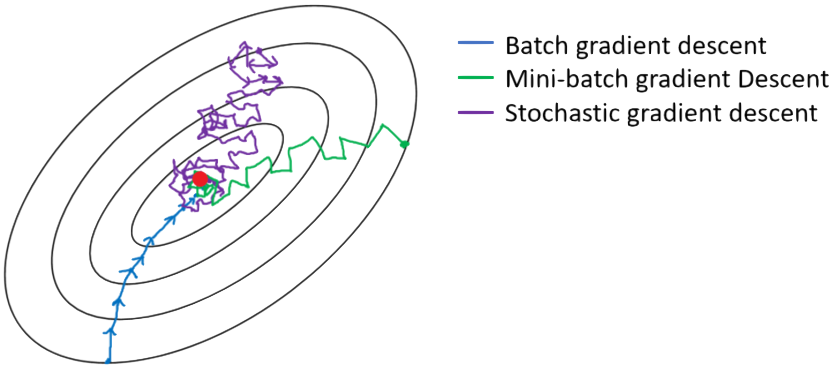
\includegraphics[width=.7\textwidth]{sgd_v_batch.png}
	\end{center}
\begin{itemize}
	\item For small batch size $s$, mini-batch gradients are nearly as fast to compute as stochastic gradients (due to parallelism).  
	\item Overall faster convergence (fewer iterations needed). 
\end{itemize}
	
\end{frame}

\end{document} 


